\documentclass[12pt]{article}
\usepackage[letterpaper, top=17mm, bottom=16mm, left=13mm, right=13mm, headheight=15pt, headsep=4mm, footskip=8mm]{geometry}
\usepackage[T1]{fontenc}
\usepackage{helvet}
\renewcommand{\familydefault}{\sfdefault}
\usepackage{tikz}
\usetikzlibrary{arrows.meta, decorations.markings}
\tikzset{midarrow/.style={postaction={decorate}, decoration={markings, mark=at position 0.5 with {\arrow{Stealth[length=3.6mm, width=3.2mm]}}}}}
\tikzset{smallarrow/.style={postaction={decorate}, decoration={markings, mark=at position 0.5 with {\arrow{Stealth[length=2.6mm, width=2.3mm]}}}}}
\tikzset{bigarrow/.style={-{Stealth[length=3mm, width=2.6mm]}, line width=1.1pt}}
\usepackage{fancyhdr}
\pagestyle{fancy}
\fancyhf{}
\lhead{\normalsize Week 62 / Conflict networks / Grades 4--5}
\lfoot{\small Bellingham Math Circle / Week 62 / W62-RV-U-v1}
\rfoot{\small \thepage}
\renewcommand{\headrulewidth}{0pt}
\setlength{\parindent}{0pt}
\setlength{\parskip}{0pt}
\raggedright
\begin{document}
\noindent\begin{minipage}[c]{0.64\linewidth}\raggedright The headers show which colour goes with each number. Put one counter on each circle. Two circles joined by a line must not get the same number. When numbers are printed next to a circle, its counter must be one of them.\end{minipage}\hfill\begin{minipage}[c]{0.33\linewidth}\raggedleft 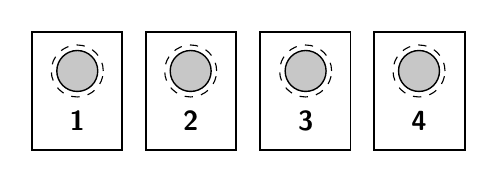
\begin{tikzpicture}[x=1mm, y=1mm]
\useasboundingbox (-0.5,-0.5) rectangle (55.5,15.5);
\draw[line width=0.7pt, fill=white] (0.0,0.0) rectangle (11.5,15.0);
\draw[dashed, line width=0.4pt] (5.8,10.0) circle (3.3mm);
\draw[line width=0.5pt, fill=black!22] (5.8,10.0) circle (2.6mm);
\node[font=\bfseries] at (5.8,3.6) {1};
\draw[line width=0.7pt, fill=white] (14.5,0.0) rectangle (26.0,15.0);
\draw[dashed, line width=0.4pt] (20.2,10.0) circle (3.3mm);
\draw[line width=0.5pt, fill=black!22] (20.2,10.0) circle (2.6mm);
\node[font=\bfseries] at (20.2,3.6) {2};
\draw[line width=0.7pt, fill=white] (29.0,0.0) rectangle (40.5,15.0);
\draw[dashed, line width=0.4pt] (34.8,10.0) circle (3.3mm);
\draw[line width=0.5pt, fill=black!22] (34.8,10.0) circle (2.6mm);
\node[font=\bfseries] at (34.8,3.6) {3};
\draw[line width=0.7pt, fill=white] (43.5,0.0) rectangle (55.0,15.0);
\draw[dashed, line width=0.4pt] (49.2,10.0) circle (3.3mm);
\draw[line width=0.5pt, fill=black!22] (49.2,10.0) circle (2.6mm);
\node[font=\bfseries] at (49.2,3.6) {4};
\end{tikzpicture}\end{minipage}\par
\vspace{4mm}
\noindent\makebox[\linewidth][c]{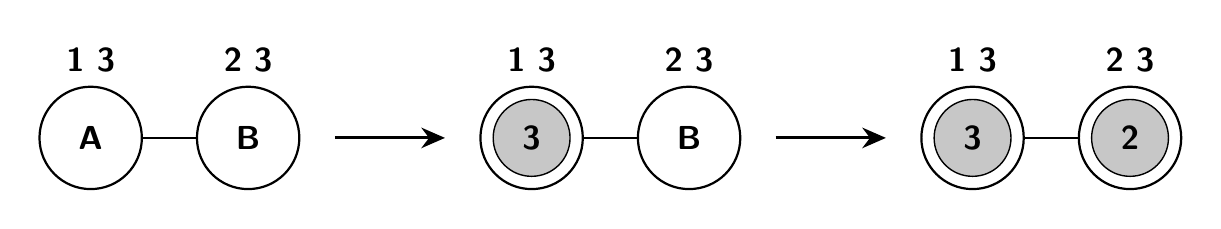
\begin{tikzpicture}[x=1mm, y=1mm]
\useasboundingbox (-8.0,-8.0) rectangle (140.0,14.0);
\draw[line width=0.8pt] (0.00,0.00) -- (20.00,0.00);
\draw[line width=0.8pt, fill=white] (0.00,0.00) circle (6.5mm);
\node[font=\large\bfseries] at (0.00,0.00) {A};
\draw[line width=0.8pt, fill=white] (20.00,0.00) circle (6.5mm);
\node[font=\large\bfseries] at (20.00,0.00) {B};
\node[font=\large\bfseries, inner sep=0.5mm, anchor=270] at (0.00,7.90) {1\,\,3};
\node[font=\large\bfseries, inner sep=0.5mm, anchor=270] at (20.00,7.90) {2\,\,3};
\draw[bigarrow] (31.0,0) -- (45.0,0);
\draw[line width=0.8pt] (56.00,0.00) -- (76.00,0.00);
\draw[line width=0.8pt, fill=white] (56.00,0.00) circle (6.5mm);
\draw[line width=0.5pt, fill=black!22] (56.00,0.00) circle (4.88mm);
\node[font=\large\bfseries] at (56.00,0.00) {3};
\draw[line width=0.8pt, fill=white] (76.00,0.00) circle (6.5mm);
\node[font=\large\bfseries] at (76.00,0.00) {B};
\node[font=\large\bfseries, inner sep=0.5mm, anchor=270] at (56.00,7.90) {1\,\,3};
\node[font=\large\bfseries, inner sep=0.5mm, anchor=270] at (76.00,7.90) {2\,\,3};
\draw[bigarrow] (87.0,0) -- (101.0,0);
\draw[line width=0.8pt] (112.00,0.00) -- (132.00,0.00);
\draw[line width=0.8pt, fill=white] (112.00,0.00) circle (6.5mm);
\draw[line width=0.5pt, fill=black!22] (112.00,0.00) circle (4.88mm);
\node[font=\large\bfseries] at (112.00,0.00) {3};
\draw[line width=0.8pt, fill=white] (132.00,0.00) circle (6.5mm);
\draw[line width=0.5pt, fill=black!22] (132.00,0.00) circle (4.88mm);
\node[font=\large\bfseries] at (132.00,0.00) {2};
\node[font=\large\bfseries, inner sep=0.5mm, anchor=270] at (112.00,7.90) {1\,\,3};
\node[font=\large\bfseries, inner sep=0.5mm, anchor=270] at (132.00,7.90) {2\,\,3};
\end{tikzpicture}}\par
\vspace{4mm}
\textbf{Problem 1:} Which of these can be done? For any that can't, explain why.\par
\vspace{5mm}
\noindent\makebox[\linewidth][c]{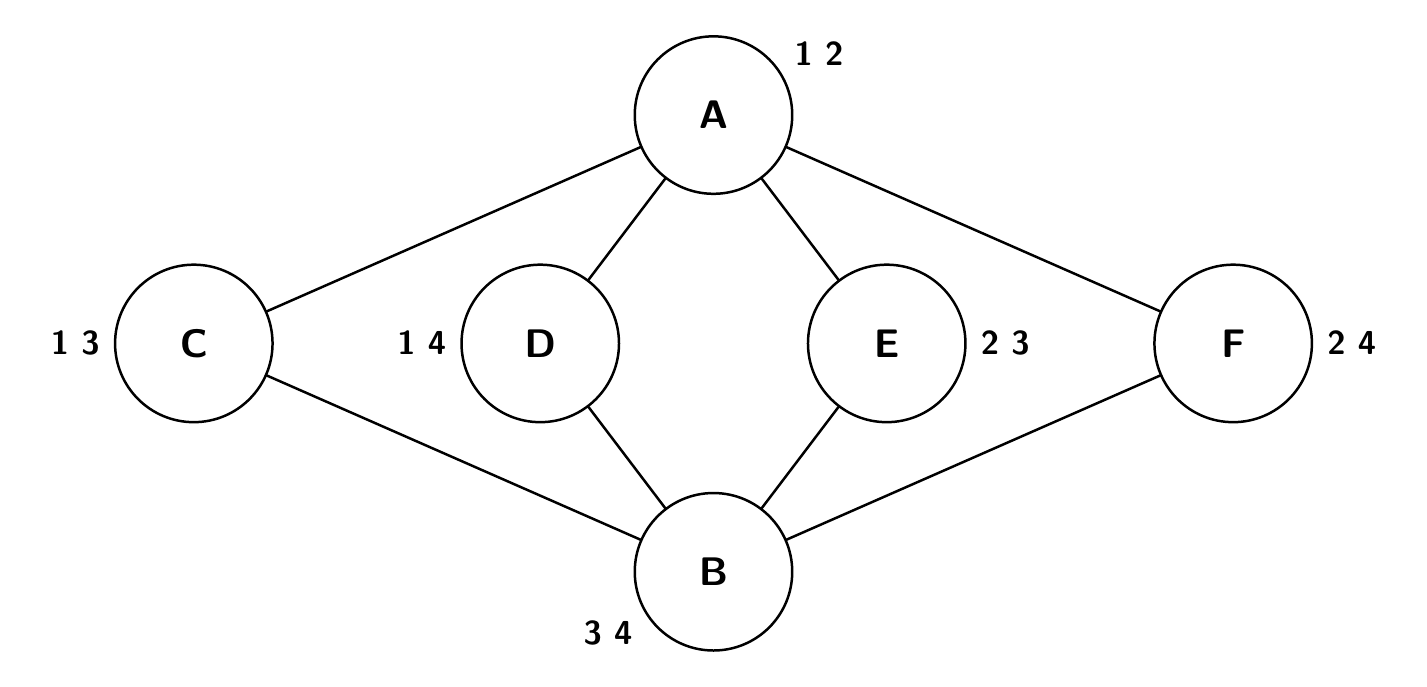
\begin{tikzpicture}[x=1mm, y=1mm]
\useasboundingbox (-87.1,-40.1) rectangle (87.1,40.1);
\draw[line width=0.9pt] (0.00,29.00) -- (-66.00,0.00);
\draw[line width=0.9pt] (0.00,29.00) -- (-22.00,0.00);
\draw[line width=0.9pt] (0.00,29.00) -- (22.00,0.00);
\draw[line width=0.9pt] (0.00,29.00) -- (66.00,0.00);
\draw[line width=0.9pt] (0.00,-29.00) -- (-66.00,0.00);
\draw[line width=0.9pt] (0.00,-29.00) -- (-22.00,0.00);
\draw[line width=0.9pt] (0.00,-29.00) -- (22.00,0.00);
\draw[line width=0.9pt] (0.00,-29.00) -- (66.00,0.00);
\draw[line width=0.9pt, fill=white] (0.00,29.00) circle (10.0mm);
\node[font=\Large\bfseries] at (0.00,29.00) {A};
\draw[line width=0.9pt, fill=white] (0.00,-29.00) circle (10.0mm);
\node[font=\Large\bfseries] at (0.00,-29.00) {B};
\draw[line width=0.9pt, fill=white] (-66.00,0.00) circle (10.0mm);
\node[font=\Large\bfseries] at (-66.00,0.00) {C};
\draw[line width=0.9pt, fill=white] (-22.00,0.00) circle (10.0mm);
\node[font=\Large\bfseries] at (-22.00,0.00) {D};
\draw[line width=0.9pt, fill=white] (22.00,0.00) circle (10.0mm);
\node[font=\Large\bfseries] at (22.00,0.00) {E};
\draw[line width=0.9pt, fill=white] (66.00,0.00) circle (10.0mm);
\node[font=\Large\bfseries] at (66.00,0.00) {F};
\node[font=\large\bfseries, inner sep=0.5mm, anchor=210] at (9.87,34.70) {1\,\,2};
\node[font=\large\bfseries, inner sep=0.5mm, anchor=30] at (-9.87,-34.70) {3\,\,4};
\node[font=\large\bfseries, inner sep=0.5mm, anchor=0] at (-77.40,0.00) {1\,\,3};
\node[font=\large\bfseries, inner sep=0.5mm, anchor=0] at (-33.40,0.00) {1\,\,4};
\node[font=\large\bfseries, inner sep=0.5mm, anchor=180] at (33.40,0.00) {2\,\,3};
\node[font=\large\bfseries, inner sep=0.5mm, anchor=180] at (77.40,0.00) {2\,\,4};
\end{tikzpicture}}\par
\vspace{11mm}
\noindent\makebox[\linewidth][c]{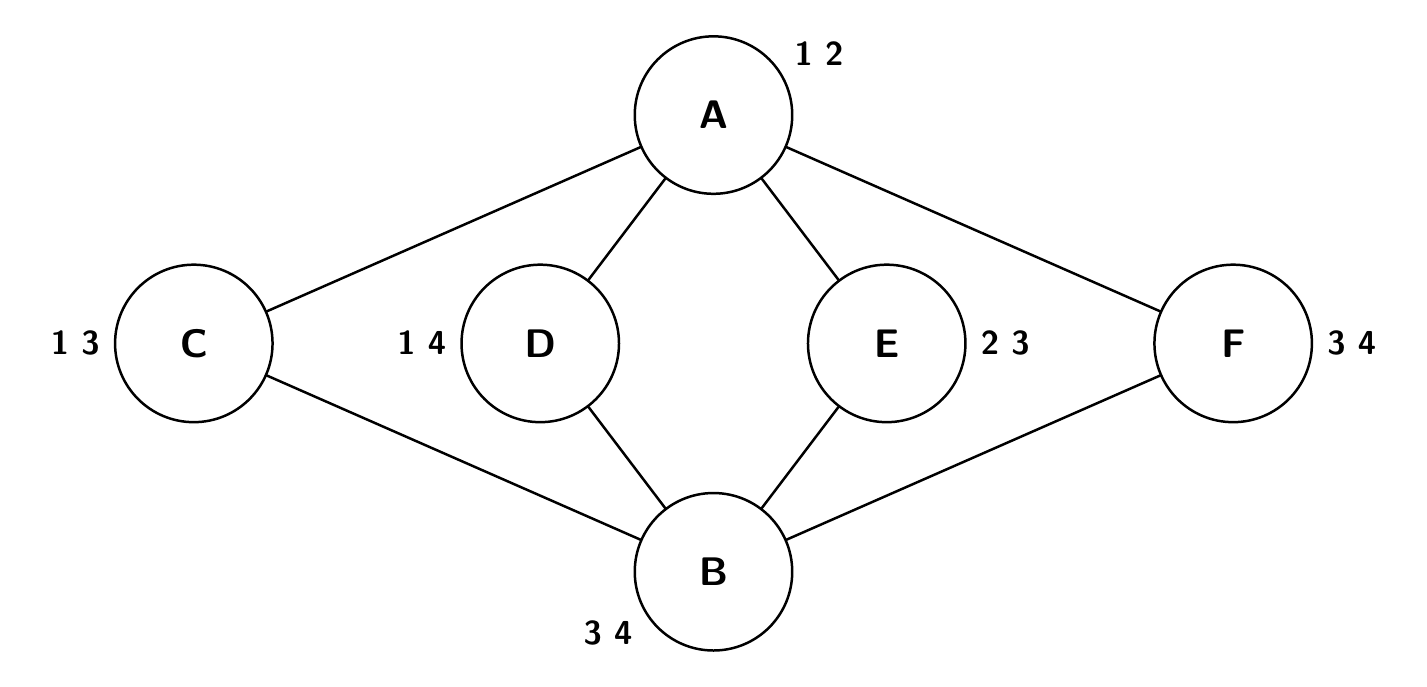
\begin{tikzpicture}[x=1mm, y=1mm]
\useasboundingbox (-87.1,-40.1) rectangle (87.1,40.1);
\draw[line width=0.9pt] (0.00,29.00) -- (-66.00,0.00);
\draw[line width=0.9pt] (0.00,29.00) -- (-22.00,0.00);
\draw[line width=0.9pt] (0.00,29.00) -- (22.00,0.00);
\draw[line width=0.9pt] (0.00,29.00) -- (66.00,0.00);
\draw[line width=0.9pt] (0.00,-29.00) -- (-66.00,0.00);
\draw[line width=0.9pt] (0.00,-29.00) -- (-22.00,0.00);
\draw[line width=0.9pt] (0.00,-29.00) -- (22.00,0.00);
\draw[line width=0.9pt] (0.00,-29.00) -- (66.00,0.00);
\draw[line width=0.9pt, fill=white] (0.00,29.00) circle (10.0mm);
\node[font=\Large\bfseries] at (0.00,29.00) {A};
\draw[line width=0.9pt, fill=white] (0.00,-29.00) circle (10.0mm);
\node[font=\Large\bfseries] at (0.00,-29.00) {B};
\draw[line width=0.9pt, fill=white] (-66.00,0.00) circle (10.0mm);
\node[font=\Large\bfseries] at (-66.00,0.00) {C};
\draw[line width=0.9pt, fill=white] (-22.00,0.00) circle (10.0mm);
\node[font=\Large\bfseries] at (-22.00,0.00) {D};
\draw[line width=0.9pt, fill=white] (22.00,0.00) circle (10.0mm);
\node[font=\Large\bfseries] at (22.00,0.00) {E};
\draw[line width=0.9pt, fill=white] (66.00,0.00) circle (10.0mm);
\node[font=\Large\bfseries] at (66.00,0.00) {F};
\node[font=\large\bfseries, inner sep=0.5mm, anchor=210] at (9.87,34.70) {1\,\,2};
\node[font=\large\bfseries, inner sep=0.5mm, anchor=30] at (-9.87,-34.70) {3\,\,4};
\node[font=\large\bfseries, inner sep=0.5mm, anchor=0] at (-77.40,0.00) {1\,\,3};
\node[font=\large\bfseries, inner sep=0.5mm, anchor=0] at (-33.40,0.00) {1\,\,4};
\node[font=\large\bfseries, inner sep=0.5mm, anchor=180] at (33.40,0.00) {2\,\,3};
\node[font=\large\bfseries, inner sep=0.5mm, anchor=180] at (77.40,0.00) {3\,\,4};
\end{tikzpicture}}\par
\newpage
\textbf{Problem 2:} Can you write two of the numbers 1, 2, 3, 4 next to every circle of this network so that it can't be done? Explain.\par
\vspace{2mm}
\noindent\makebox[\linewidth][c]{\begin{tikzpicture}[x=1mm, y=1mm]
\useasboundingbox (-62.0,-49.0) rectangle (62.0,49.0);
\draw[line width=0.9pt] (0.00,32.00) -- (-38.00,0.00);
\draw[line width=0.9pt] (0.00,32.00) -- (0.00,0.00);
\draw[line width=0.9pt] (0.00,32.00) -- (38.00,0.00);
\draw[line width=0.9pt] (0.00,-32.00) -- (-38.00,0.00);
\draw[line width=0.9pt] (0.00,-32.00) -- (0.00,0.00);
\draw[line width=0.9pt] (0.00,-32.00) -- (38.00,0.00);
\draw[line width=0.9pt, fill=white] (0.00,32.00) circle (10.0mm);
\node[font=\Large\bfseries] at (0.00,32.00) {A};
\draw[line width=0.9pt, fill=white] (0.00,-32.00) circle (10.0mm);
\node[font=\Large\bfseries] at (0.00,-32.00) {B};
\draw[line width=0.9pt, fill=white] (-38.00,0.00) circle (10.0mm);
\node[font=\Large\bfseries] at (-38.00,0.00) {C};
\draw[line width=0.9pt, fill=white] (0.00,0.00) circle (10.0mm);
\node[font=\Large\bfseries] at (0.00,0.00) {D};
\draw[line width=0.9pt, fill=white] (38.00,0.00) circle (10.0mm);
\node[font=\Large\bfseries] at (38.00,0.00) {E};
\end{tikzpicture}}\par
\vspace{8mm}
\textbf{Problem 3:} Can you write two of the numbers 1, 2, 3, 4 next to every circle of this tree so that it can't be done? Explain.\par
\vspace{2mm}
\noindent\makebox[\linewidth][c]{\begin{tikzpicture}[x=1mm, y=1mm]
\useasboundingbox (-92.0,-49.0) rectangle (92.0,49.0);
\draw[line width=0.9pt] (0.00,0.00) -- (0.00,32.00);
\draw[line width=0.9pt] (0.00,0.00) -- (-34.00,0.00);
\draw[line width=0.9pt] (-34.00,0.00) -- (-68.00,0.00);
\draw[line width=0.9pt] (0.00,0.00) -- (34.00,0.00);
\draw[line width=0.9pt] (34.00,0.00) -- (34.00,-32.00);
\draw[line width=0.9pt] (34.00,0.00) -- (68.00,0.00);
\draw[line width=0.9pt] (68.00,0.00) -- (68.00,32.00);
\draw[line width=0.9pt, fill=white] (0.00,32.00) circle (10.0mm);
\node[font=\Large\bfseries] at (0.00,32.00) {A};
\draw[line width=0.9pt, fill=white] (0.00,0.00) circle (10.0mm);
\node[font=\Large\bfseries] at (0.00,0.00) {H};
\draw[line width=0.9pt, fill=white] (-34.00,0.00) circle (10.0mm);
\node[font=\Large\bfseries] at (-34.00,0.00) {B};
\draw[line width=0.9pt, fill=white] (-68.00,0.00) circle (10.0mm);
\node[font=\Large\bfseries] at (-68.00,0.00) {C};
\draw[line width=0.9pt, fill=white] (34.00,0.00) circle (10.0mm);
\node[font=\Large\bfseries] at (34.00,0.00) {D};
\draw[line width=0.9pt, fill=white] (34.00,-32.00) circle (10.0mm);
\node[font=\Large\bfseries] at (34.00,-32.00) {E};
\draw[line width=0.9pt, fill=white] (68.00,0.00) circle (10.0mm);
\node[font=\Large\bfseries] at (68.00,0.00) {F};
\draw[line width=0.9pt, fill=white] (68.00,32.00) circle (10.0mm);
\node[font=\Large\bfseries] at (68.00,32.00) {G};
\end{tikzpicture}}\par
\newpage
\textbf{Problem 4:} Which of these can be done? Suppose every circle of a ring, of any size, has two numbers next to it. When can it not be done? Explain.\par
\vspace{8mm}
\noindent\makebox[\linewidth][s]{\hfill 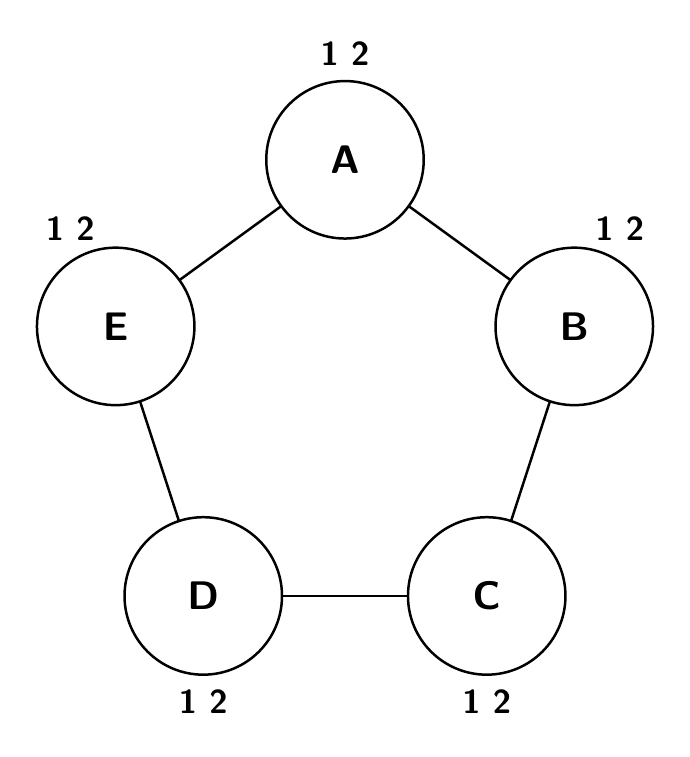
\begin{tikzpicture}[x=1mm, y=1mm]
\useasboundingbox (-40.3,-41.6) rectangle (40.3,47.4);
\draw[line width=0.9pt] (0.00,30.62) -- (29.12,9.46);
\draw[line width=0.9pt] (29.12,9.46) -- (18.00,-24.77);
\draw[line width=0.9pt] (18.00,-24.77) -- (-18.00,-24.77);
\draw[line width=0.9pt] (-18.00,-24.77) -- (-29.12,9.46);
\draw[line width=0.9pt] (-29.12,9.46) -- (0.00,30.62);
\draw[line width=0.9pt, fill=white] (0.00,30.62) circle (10.0mm);
\node[font=\Large\bfseries] at (0.00,30.62) {A};
\draw[line width=0.9pt, fill=white] (29.12,9.46) circle (10.0mm);
\node[font=\Large\bfseries] at (29.12,9.46) {B};
\draw[line width=0.9pt, fill=white] (18.00,-24.77) circle (10.0mm);
\node[font=\Large\bfseries] at (18.00,-24.77) {C};
\draw[line width=0.9pt, fill=white] (-18.00,-24.77) circle (10.0mm);
\node[font=\Large\bfseries] at (-18.00,-24.77) {D};
\draw[line width=0.9pt, fill=white] (-29.12,9.46) circle (10.0mm);
\node[font=\Large\bfseries] at (-29.12,9.46) {E};
\node[font=\large\bfseries, inner sep=0.5mm, anchor=270] at (0.00,42.02) {1\,\,2};
\node[font=\large\bfseries, inner sep=0.5mm, anchor=245] at (33.94,19.80) {1\,\,2};
\node[font=\large\bfseries, inner sep=0.5mm, anchor=90] at (18.00,-36.17) {1\,\,2};
\node[font=\large\bfseries, inner sep=0.5mm, anchor=90] at (-18.00,-36.17) {1\,\,2};
\node[font=\large\bfseries, inner sep=0.5mm, anchor=295] at (-33.94,19.80) {1\,\,2};
\end{tikzpicture} \hfill 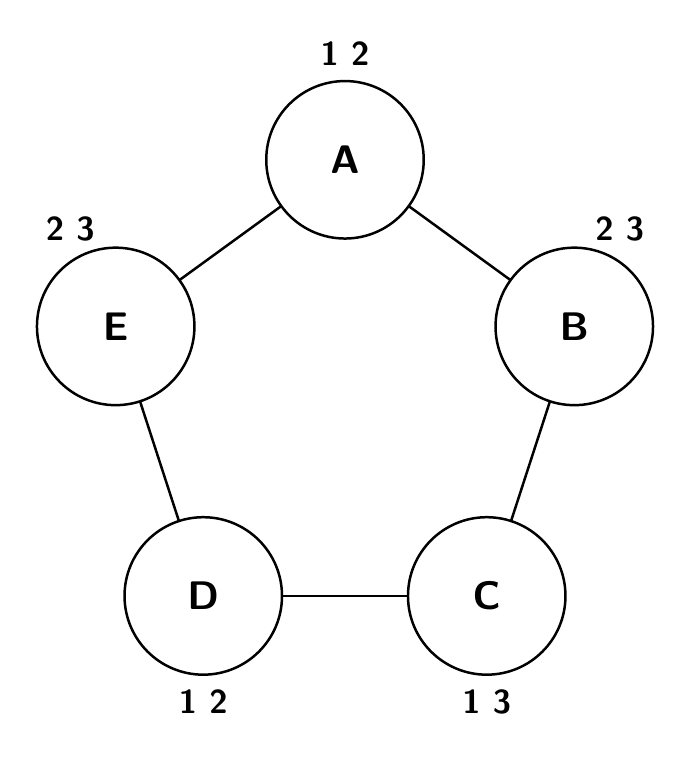
\begin{tikzpicture}[x=1mm, y=1mm]
\useasboundingbox (-40.3,-41.6) rectangle (40.3,47.4);
\draw[line width=0.9pt] (0.00,30.62) -- (29.12,9.46);
\draw[line width=0.9pt] (29.12,9.46) -- (18.00,-24.77);
\draw[line width=0.9pt] (18.00,-24.77) -- (-18.00,-24.77);
\draw[line width=0.9pt] (-18.00,-24.77) -- (-29.12,9.46);
\draw[line width=0.9pt] (-29.12,9.46) -- (0.00,30.62);
\draw[line width=0.9pt, fill=white] (0.00,30.62) circle (10.0mm);
\node[font=\Large\bfseries] at (0.00,30.62) {A};
\draw[line width=0.9pt, fill=white] (29.12,9.46) circle (10.0mm);
\node[font=\Large\bfseries] at (29.12,9.46) {B};
\draw[line width=0.9pt, fill=white] (18.00,-24.77) circle (10.0mm);
\node[font=\Large\bfseries] at (18.00,-24.77) {C};
\draw[line width=0.9pt, fill=white] (-18.00,-24.77) circle (10.0mm);
\node[font=\Large\bfseries] at (-18.00,-24.77) {D};
\draw[line width=0.9pt, fill=white] (-29.12,9.46) circle (10.0mm);
\node[font=\Large\bfseries] at (-29.12,9.46) {E};
\node[font=\large\bfseries, inner sep=0.5mm, anchor=270] at (0.00,42.02) {1\,\,2};
\node[font=\large\bfseries, inner sep=0.5mm, anchor=245] at (33.94,19.80) {2\,\,3};
\node[font=\large\bfseries, inner sep=0.5mm, anchor=90] at (18.00,-36.17) {1\,\,3};
\node[font=\large\bfseries, inner sep=0.5mm, anchor=90] at (-18.00,-36.17) {1\,\,2};
\node[font=\large\bfseries, inner sep=0.5mm, anchor=295] at (-33.94,19.80) {2\,\,3};
\end{tikzpicture} \hfill}\par
\vspace{12mm}
\noindent\makebox[\linewidth][s]{\hfill 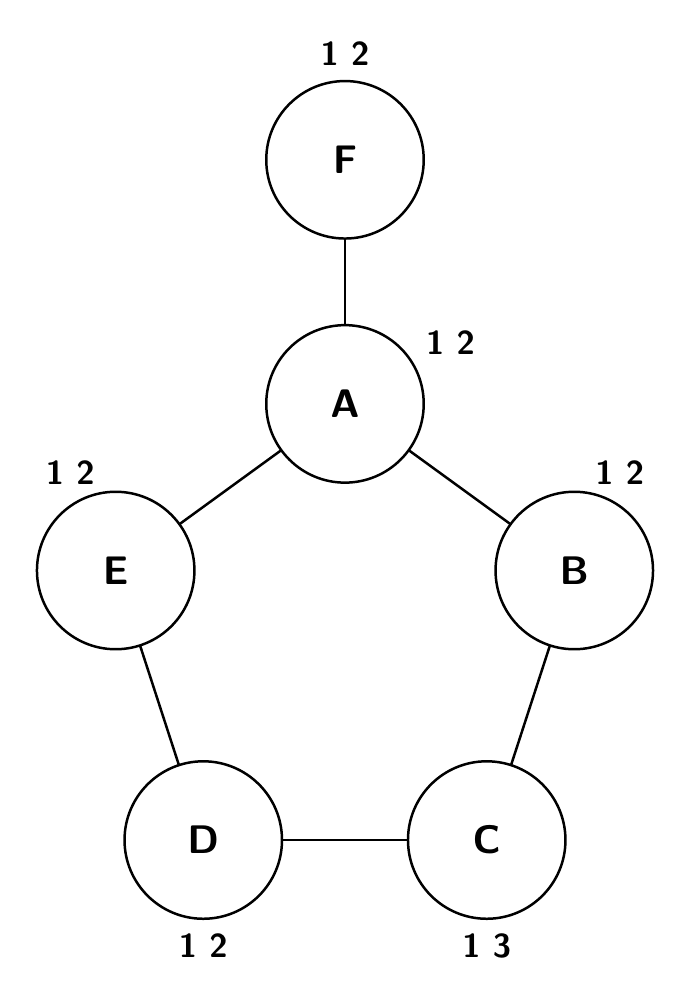
\begin{tikzpicture}[x=1mm, y=1mm]
\useasboundingbox (-40.3,-41.6) rectangle (40.3,78.4);
\draw[line width=0.9pt] (0.00,30.62) -- (29.12,9.46);
\draw[line width=0.9pt] (29.12,9.46) -- (18.00,-24.77);
\draw[line width=0.9pt] (18.00,-24.77) -- (-18.00,-24.77);
\draw[line width=0.9pt] (-18.00,-24.77) -- (-29.12,9.46);
\draw[line width=0.9pt] (-29.12,9.46) -- (0.00,30.62);
\draw[line width=0.9pt] (0.00,30.62) -- (0.00,61.62);
\draw[line width=0.9pt, fill=white] (0.00,30.62) circle (10.0mm);
\node[font=\Large\bfseries] at (0.00,30.62) {A};
\draw[line width=0.9pt, fill=white] (29.12,9.46) circle (10.0mm);
\node[font=\Large\bfseries] at (29.12,9.46) {B};
\draw[line width=0.9pt, fill=white] (18.00,-24.77) circle (10.0mm);
\node[font=\Large\bfseries] at (18.00,-24.77) {C};
\draw[line width=0.9pt, fill=white] (-18.00,-24.77) circle (10.0mm);
\node[font=\Large\bfseries] at (-18.00,-24.77) {D};
\draw[line width=0.9pt, fill=white] (-29.12,9.46) circle (10.0mm);
\node[font=\Large\bfseries] at (-29.12,9.46) {E};
\draw[line width=0.9pt, fill=white] (0.00,61.62) circle (10.0mm);
\node[font=\Large\bfseries] at (0.00,61.62) {F};
\node[font=\large\bfseries, inner sep=0.5mm, anchor=210] at (9.87,36.32) {1\,\,2};
\node[font=\large\bfseries, inner sep=0.5mm, anchor=245] at (33.94,19.80) {1\,\,2};
\node[font=\large\bfseries, inner sep=0.5mm, anchor=90] at (18.00,-36.17) {1\,\,3};
\node[font=\large\bfseries, inner sep=0.5mm, anchor=90] at (-18.00,-36.17) {1\,\,2};
\node[font=\large\bfseries, inner sep=0.5mm, anchor=295] at (-33.94,19.80) {1\,\,2};
\node[font=\large\bfseries, inner sep=0.5mm, anchor=270] at (0.00,73.02) {1\,\,2};
\end{tikzpicture} \hfill 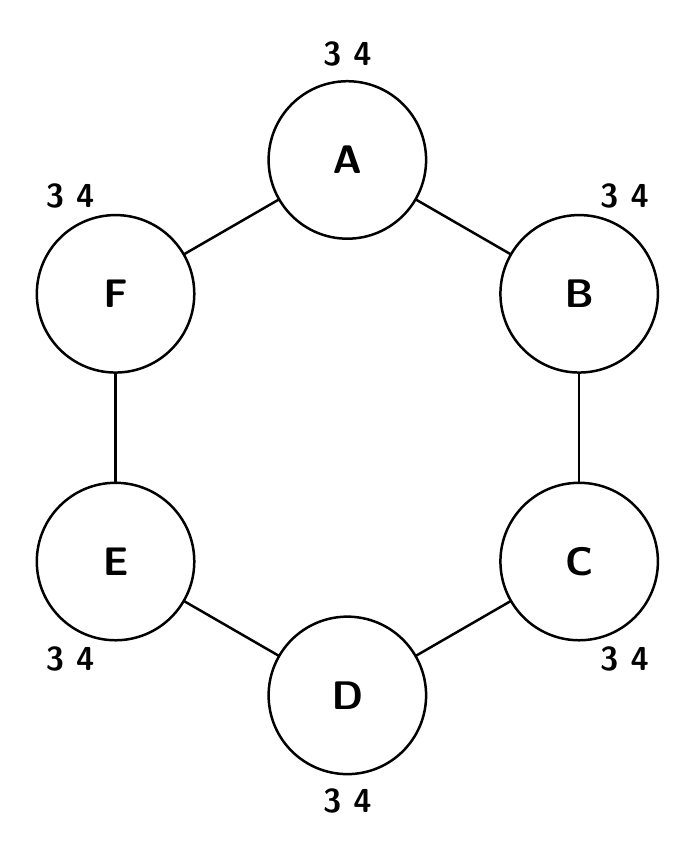
\begin{tikzpicture}[x=1mm, y=1mm]
\useasboundingbox (-40.6,-50.8) rectangle (40.6,50.8);
\draw[line width=0.9pt] (0.00,34.00) -- (29.44,17.00);
\draw[line width=0.9pt] (29.44,17.00) -- (29.44,-17.00);
\draw[line width=0.9pt] (29.44,-17.00) -- (0.00,-34.00);
\draw[line width=0.9pt] (0.00,-34.00) -- (-29.44,-17.00);
\draw[line width=0.9pt] (-29.44,-17.00) -- (-29.44,17.00);
\draw[line width=0.9pt] (-29.44,17.00) -- (0.00,34.00);
\draw[line width=0.9pt, fill=white] (0.00,34.00) circle (10.0mm);
\node[font=\Large\bfseries] at (0.00,34.00) {A};
\draw[line width=0.9pt, fill=white] (29.44,17.00) circle (10.0mm);
\node[font=\Large\bfseries] at (29.44,17.00) {B};
\draw[line width=0.9pt, fill=white] (29.44,-17.00) circle (10.0mm);
\node[font=\Large\bfseries] at (29.44,-17.00) {C};
\draw[line width=0.9pt, fill=white] (0.00,-34.00) circle (10.0mm);
\node[font=\Large\bfseries] at (0.00,-34.00) {D};
\draw[line width=0.9pt, fill=white] (-29.44,-17.00) circle (10.0mm);
\node[font=\Large\bfseries] at (-29.44,-17.00) {E};
\draw[line width=0.9pt, fill=white] (-29.44,17.00) circle (10.0mm);
\node[font=\Large\bfseries] at (-29.44,17.00) {F};
\node[font=\large\bfseries, inner sep=0.5mm, anchor=270] at (0.00,45.40) {3\,\,4};
\node[font=\large\bfseries, inner sep=0.5mm, anchor=245] at (34.26,27.33) {3\,\,4};
\node[font=\large\bfseries, inner sep=0.5mm, anchor=115] at (34.26,-27.33) {3\,\,4};
\node[font=\large\bfseries, inner sep=0.5mm, anchor=90] at (-0.00,-45.40) {3\,\,4};
\node[font=\large\bfseries, inner sep=0.5mm, anchor=65] at (-34.26,-27.33) {3\,\,4};
\node[font=\large\bfseries, inner sep=0.5mm, anchor=295] at (-34.26,27.33) {3\,\,4};
\end{tikzpicture} \hfill}\par
\newpage
A move takes one counter off a circle and puts a counter with a different number there. After every move, no line may have the same number at both ends. Write a move as the circle's letter and its new number, like D1.\par
\vspace{3mm}
\noindent\makebox[\linewidth][c]{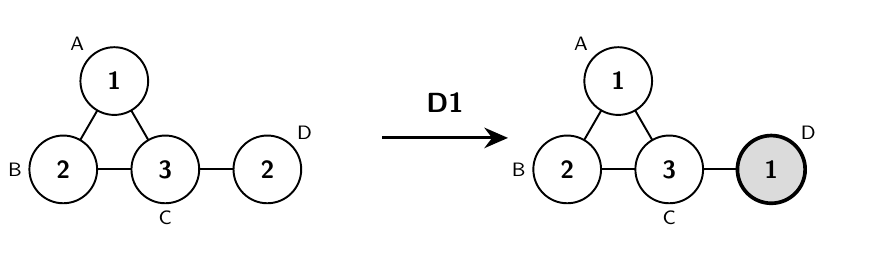
\begin{tikzpicture}[x=1mm, y=1mm]
\useasboundingbox (-11.0,-7.0) rectangle (95.0,18.0);
\draw[line width=0.7pt] (0.00,11.22) -- (-6.48,0.00);
\draw[line width=0.7pt] (-6.48,0.00) -- (6.48,0.00);
\draw[line width=0.7pt] (6.48,0.00) -- (0.00,11.22);
\draw[line width=0.7pt] (6.48,0.00) -- (19.44,0.00);
\draw[line width=0.7pt, fill=white] (0.00,11.22) circle (4.3mm);
\node[font=\small\bfseries] at (0.00,11.22) {1};
\node[font=\scriptsize, inner sep=0.4mm, anchor=315] at (-3.39,14.62) {A};
\draw[line width=0.7pt, fill=white] (-6.48,0.00) circle (4.3mm);
\node[font=\small\bfseries] at (-6.48,0.00) {2};
\node[font=\scriptsize, inner sep=0.4mm, anchor=0] at (-11.28,0.00) {B};
\draw[line width=0.7pt, fill=white] (6.48,0.00) circle (4.3mm);
\node[font=\small\bfseries] at (6.48,0.00) {3};
\node[font=\scriptsize, inner sep=0.4mm, anchor=90] at (6.48,-4.80) {C};
\draw[line width=0.7pt, fill=white] (19.44,0.00) circle (4.3mm);
\node[font=\small\bfseries] at (19.44,0.00) {2};
\node[font=\scriptsize, inner sep=0.4mm, anchor=225] at (22.83,3.39) {D};
\draw[bigarrow] (34.0,4) -- (50.0,4);
\node[font=\bfseries] at (42.0,8.5) {D1};
\draw[line width=0.7pt] (64.00,11.22) -- (57.52,0.00);
\draw[line width=0.7pt] (57.52,0.00) -- (70.48,0.00);
\draw[line width=0.7pt] (70.48,0.00) -- (64.00,11.22);
\draw[line width=0.7pt] (70.48,0.00) -- (83.44,0.00);
\draw[line width=0.7pt, fill=white] (64.00,11.22) circle (4.3mm);
\node[font=\small\bfseries] at (64.00,11.22) {1};
\node[font=\scriptsize, inner sep=0.4mm, anchor=315] at (60.61,14.62) {A};
\draw[line width=0.7pt, fill=white] (57.52,0.00) circle (4.3mm);
\node[font=\small\bfseries] at (57.52,0.00) {2};
\node[font=\scriptsize, inner sep=0.4mm, anchor=0] at (52.72,0.00) {B};
\draw[line width=0.7pt, fill=white] (70.48,0.00) circle (4.3mm);
\node[font=\small\bfseries] at (70.48,0.00) {3};
\node[font=\scriptsize, inner sep=0.4mm, anchor=90] at (70.48,-4.80) {C};
\draw[line width=1.3299999999999998pt, fill=black!14] (83.44,0.00) circle (4.3mm);
\node[font=\small\bfseries] at (83.44,0.00) {1};
\node[font=\scriptsize, inner sep=0.4mm, anchor=225] at (86.83,3.39) {D};
\end{tikzpicture}}\par
\vspace{3mm}
\textbf{Problem 5:} Using only the counters shown, can you change Start into Goal? Write the fewest moves you can find, or explain why it can't be done.\par
\vspace{6mm}
\noindent\makebox[\linewidth][c]{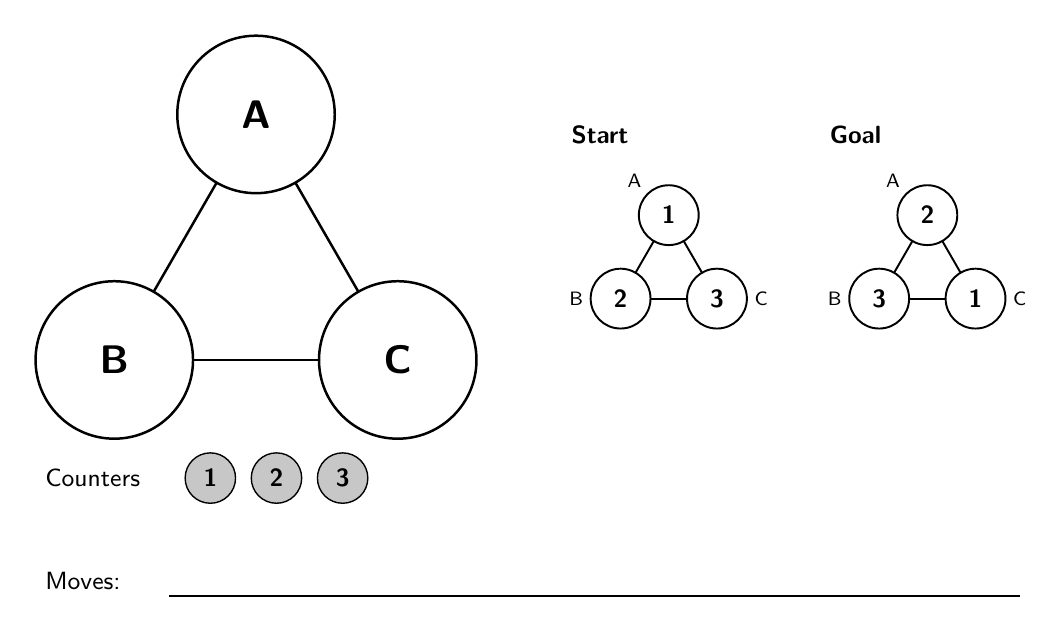
\begin{tikzpicture}[x=1mm, y=1mm]
\useasboundingbox (-29.0,-32.0) rectangle (98.7,42.2);
\draw[line width=0.9pt] (0.00,31.18) -- (-18.00,0.00);
\draw[line width=0.9pt] (-18.00,0.00) -- (18.00,0.00);
\draw[line width=0.9pt] (18.00,0.00) -- (0.00,31.18);
\draw[line width=0.9pt, fill=white] (0.00,31.18) circle (10.0mm);
\node[font=\Large\bfseries] at (0.00,31.18) {A};
\draw[line width=0.9pt, fill=white] (-18.00,0.00) circle (10.0mm);
\node[font=\Large\bfseries] at (-18.00,0.00) {B};
\draw[line width=0.9pt, fill=white] (18.00,0.00) circle (10.0mm);
\node[font=\Large\bfseries] at (18.00,0.00) {C};
\node[anchor=north west, font=\small\bfseries, inner sep=0] at (40.0,29.7) {Start};
\draw[line width=0.7pt] (52.42,18.39) -- (46.30,7.79);
\draw[line width=0.7pt] (46.30,7.79) -- (58.54,7.79);
\draw[line width=0.7pt] (58.54,7.79) -- (52.42,18.39);
\draw[line width=0.7pt, fill=white] (52.42,18.39) circle (3.8mm);
\node[font=\small\bfseries] at (52.42,18.39) {1};
\node[font=\scriptsize, inner sep=0.4mm, anchor=315] at (49.38,21.43) {A};
\draw[line width=0.7pt, fill=white] (46.30,7.79) circle (3.8mm);
\node[font=\small\bfseries] at (46.30,7.79) {2};
\node[font=\scriptsize, inner sep=0.4mm, anchor=0] at (42.00,7.79) {B};
\draw[line width=0.7pt, fill=white] (58.54,7.79) circle (3.8mm);
\node[font=\small\bfseries] at (58.54,7.79) {3};
\node[font=\scriptsize, inner sep=0.4mm, anchor=180] at (62.84,7.79) {C};
\node[anchor=north west, font=\small\bfseries, inner sep=0] at (72.8,29.7) {Goal};
\draw[line width=0.7pt] (85.26,18.39) -- (79.14,7.79);
\draw[line width=0.7pt] (79.14,7.79) -- (91.38,7.79);
\draw[line width=0.7pt] (91.38,7.79) -- (85.26,18.39);
\draw[line width=0.7pt, fill=white] (85.26,18.39) circle (3.8mm);
\node[font=\small\bfseries] at (85.26,18.39) {2};
\node[font=\scriptsize, inner sep=0.4mm, anchor=315] at (82.22,21.43) {A};
\draw[line width=0.7pt, fill=white] (79.14,7.79) circle (3.8mm);
\node[font=\small\bfseries] at (79.14,7.79) {3};
\node[font=\scriptsize, inner sep=0.4mm, anchor=0] at (74.84,7.79) {B};
\draw[line width=0.7pt, fill=white] (91.38,7.79) circle (3.8mm);
\node[font=\small\bfseries] at (91.38,7.79) {1};
\node[font=\scriptsize, inner sep=0.4mm, anchor=180] at (95.68,7.79) {C};
\node[anchor=west, font=\small] at (-28.0,-15.0) {Counters};
\draw[line width=0.5pt, fill=black!22] (-5.8,-15.0) circle (3.2mm);
\node[font=\small\bfseries] at (-5.8,-15.0) {1};
\draw[line width=0.5pt, fill=black!22] (2.6,-15.0) circle (3.2mm);
\node[font=\small\bfseries] at (2.6,-15.0) {2};
\draw[line width=0.5pt, fill=black!22] (11.0,-15.0) circle (3.2mm);
\node[font=\small\bfseries] at (11.0,-15.0) {3};
\node[anchor=west, font=\small] at (-28.0,-28.0) {Moves:};
\draw[line width=0.5pt] (-11.0,-30.0) -- (97.0,-30.0);
\end{tikzpicture}}\par
\vspace{12mm}
\noindent\makebox[\linewidth][c]{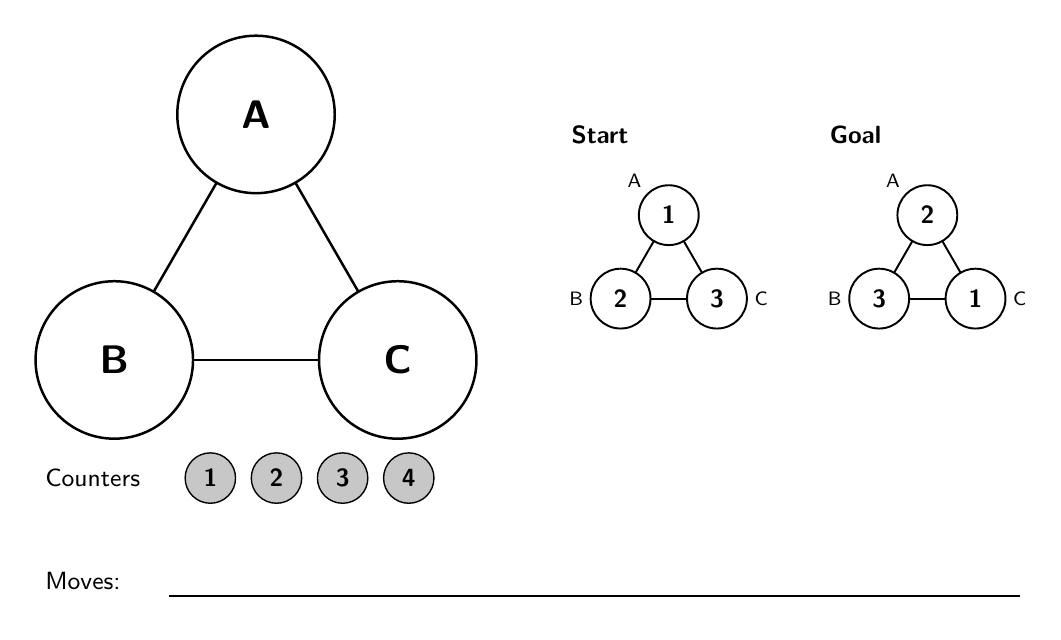
\begin{tikzpicture}[x=1mm, y=1mm]
\useasboundingbox (-29.0,-32.0) rectangle (98.7,42.2);
\draw[line width=0.9pt] (0.00,31.18) -- (-18.00,0.00);
\draw[line width=0.9pt] (-18.00,0.00) -- (18.00,0.00);
\draw[line width=0.9pt] (18.00,0.00) -- (0.00,31.18);
\draw[line width=0.9pt, fill=white] (0.00,31.18) circle (10.0mm);
\node[font=\Large\bfseries] at (0.00,31.18) {A};
\draw[line width=0.9pt, fill=white] (-18.00,0.00) circle (10.0mm);
\node[font=\Large\bfseries] at (-18.00,0.00) {B};
\draw[line width=0.9pt, fill=white] (18.00,0.00) circle (10.0mm);
\node[font=\Large\bfseries] at (18.00,0.00) {C};
\node[anchor=north west, font=\small\bfseries, inner sep=0] at (40.0,29.7) {Start};
\draw[line width=0.7pt] (52.42,18.39) -- (46.30,7.79);
\draw[line width=0.7pt] (46.30,7.79) -- (58.54,7.79);
\draw[line width=0.7pt] (58.54,7.79) -- (52.42,18.39);
\draw[line width=0.7pt, fill=white] (52.42,18.39) circle (3.8mm);
\node[font=\small\bfseries] at (52.42,18.39) {1};
\node[font=\scriptsize, inner sep=0.4mm, anchor=315] at (49.38,21.43) {A};
\draw[line width=0.7pt, fill=white] (46.30,7.79) circle (3.8mm);
\node[font=\small\bfseries] at (46.30,7.79) {2};
\node[font=\scriptsize, inner sep=0.4mm, anchor=0] at (42.00,7.79) {B};
\draw[line width=0.7pt, fill=white] (58.54,7.79) circle (3.8mm);
\node[font=\small\bfseries] at (58.54,7.79) {3};
\node[font=\scriptsize, inner sep=0.4mm, anchor=180] at (62.84,7.79) {C};
\node[anchor=north west, font=\small\bfseries, inner sep=0] at (72.8,29.7) {Goal};
\draw[line width=0.7pt] (85.26,18.39) -- (79.14,7.79);
\draw[line width=0.7pt] (79.14,7.79) -- (91.38,7.79);
\draw[line width=0.7pt] (91.38,7.79) -- (85.26,18.39);
\draw[line width=0.7pt, fill=white] (85.26,18.39) circle (3.8mm);
\node[font=\small\bfseries] at (85.26,18.39) {2};
\node[font=\scriptsize, inner sep=0.4mm, anchor=315] at (82.22,21.43) {A};
\draw[line width=0.7pt, fill=white] (79.14,7.79) circle (3.8mm);
\node[font=\small\bfseries] at (79.14,7.79) {3};
\node[font=\scriptsize, inner sep=0.4mm, anchor=0] at (74.84,7.79) {B};
\draw[line width=0.7pt, fill=white] (91.38,7.79) circle (3.8mm);
\node[font=\small\bfseries] at (91.38,7.79) {1};
\node[font=\scriptsize, inner sep=0.4mm, anchor=180] at (95.68,7.79) {C};
\node[anchor=west, font=\small] at (-28.0,-15.0) {Counters};
\draw[line width=0.5pt, fill=black!22] (-5.8,-15.0) circle (3.2mm);
\node[font=\small\bfseries] at (-5.8,-15.0) {1};
\draw[line width=0.5pt, fill=black!22] (2.6,-15.0) circle (3.2mm);
\node[font=\small\bfseries] at (2.6,-15.0) {2};
\draw[line width=0.5pt, fill=black!22] (11.0,-15.0) circle (3.2mm);
\node[font=\small\bfseries] at (11.0,-15.0) {3};
\draw[line width=0.5pt, fill=black!22] (19.4,-15.0) circle (3.2mm);
\node[font=\small\bfseries] at (19.4,-15.0) {4};
\node[anchor=west, font=\small] at (-28.0,-28.0) {Moves:};
\draw[line width=0.5pt] (-11.0,-30.0) -- (97.0,-30.0);
\end{tikzpicture}}\par
\newpage
\textbf{Problem 6:} Use counters 1, 2 and 3. On which of these rings can you place counters, with different numbers at the two ends of every line, so that no counter can move? Explain.\par
\vspace{10mm}
\noindent\makebox[\linewidth][s]{\hfill 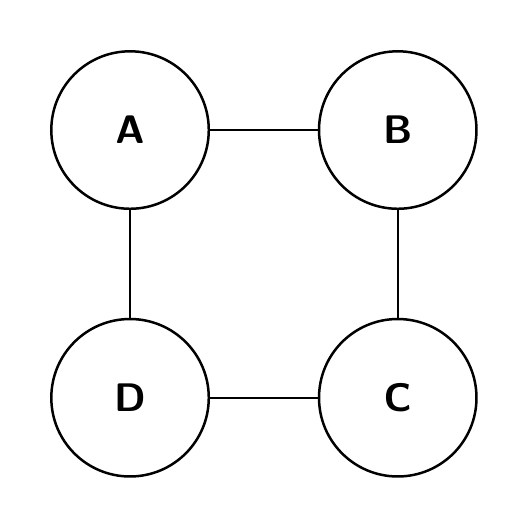
\begin{tikzpicture}[x=1mm, y=1mm]
\useasboundingbox (-30.0,-30.0) rectangle (30.0,30.0);
\draw[line width=0.9pt] (-17.00,17.00) -- (17.00,17.00);
\draw[line width=0.9pt] (17.00,17.00) -- (17.00,-17.00);
\draw[line width=0.9pt] (17.00,-17.00) -- (-17.00,-17.00);
\draw[line width=0.9pt] (-17.00,-17.00) -- (-17.00,17.00);
\draw[line width=0.9pt, fill=white] (-17.00,17.00) circle (10.0mm);
\node[font=\Large\bfseries] at (-17.00,17.00) {A};
\draw[line width=0.9pt, fill=white] (17.00,17.00) circle (10.0mm);
\node[font=\Large\bfseries] at (17.00,17.00) {B};
\draw[line width=0.9pt, fill=white] (17.00,-17.00) circle (10.0mm);
\node[font=\Large\bfseries] at (17.00,-17.00) {C};
\draw[line width=0.9pt, fill=white] (-17.00,-17.00) circle (10.0mm);
\node[font=\Large\bfseries] at (-17.00,-17.00) {D};
\end{tikzpicture} \hfill 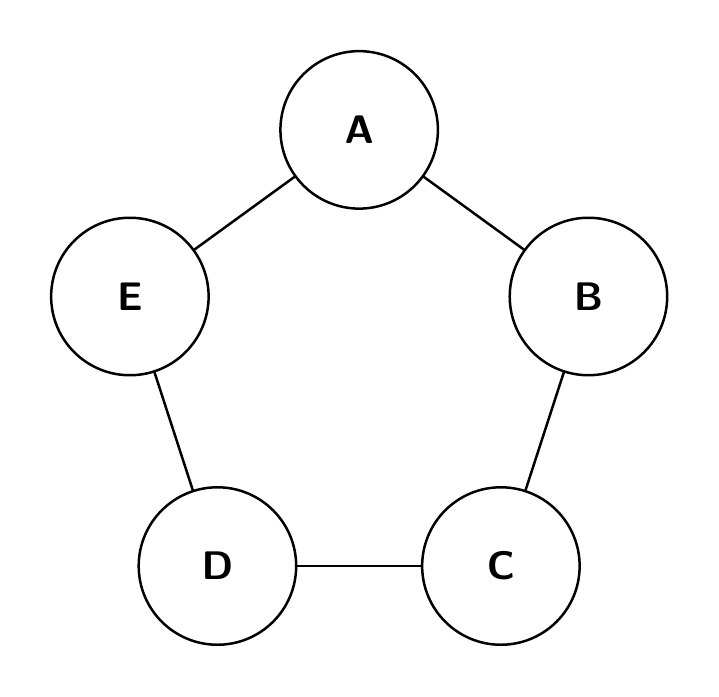
\begin{tikzpicture}[x=1mm, y=1mm]
\useasboundingbox (-42.1,-37.8) rectangle (42.1,43.6);
\draw[line width=0.9pt] (0.00,30.62) -- (29.12,9.46);
\draw[line width=0.9pt] (29.12,9.46) -- (18.00,-24.77);
\draw[line width=0.9pt] (18.00,-24.77) -- (-18.00,-24.77);
\draw[line width=0.9pt] (-18.00,-24.77) -- (-29.12,9.46);
\draw[line width=0.9pt] (-29.12,9.46) -- (0.00,30.62);
\draw[line width=0.9pt, fill=white] (0.00,30.62) circle (10.0mm);
\node[font=\Large\bfseries] at (0.00,30.62) {A};
\draw[line width=0.9pt, fill=white] (29.12,9.46) circle (10.0mm);
\node[font=\Large\bfseries] at (29.12,9.46) {B};
\draw[line width=0.9pt, fill=white] (18.00,-24.77) circle (10.0mm);
\node[font=\Large\bfseries] at (18.00,-24.77) {C};
\draw[line width=0.9pt, fill=white] (-18.00,-24.77) circle (10.0mm);
\node[font=\Large\bfseries] at (-18.00,-24.77) {D};
\draw[line width=0.9pt, fill=white] (-29.12,9.46) circle (10.0mm);
\node[font=\Large\bfseries] at (-29.12,9.46) {E};
\end{tikzpicture} \hfill}\par
\vspace{12mm}
\noindent\makebox[\linewidth][s]{\hfill 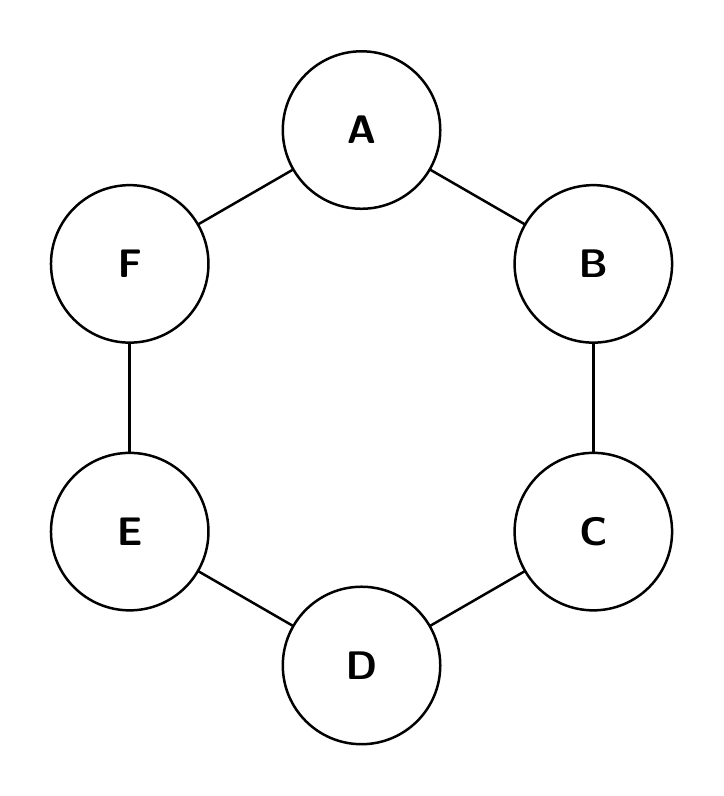
\begin{tikzpicture}[x=1mm, y=1mm]
\useasboundingbox (-42.4,-47.0) rectangle (42.4,47.0);
\draw[line width=0.9pt] (0.00,34.00) -- (29.44,17.00);
\draw[line width=0.9pt] (29.44,17.00) -- (29.44,-17.00);
\draw[line width=0.9pt] (29.44,-17.00) -- (0.00,-34.00);
\draw[line width=0.9pt] (0.00,-34.00) -- (-29.44,-17.00);
\draw[line width=0.9pt] (-29.44,-17.00) -- (-29.44,17.00);
\draw[line width=0.9pt] (-29.44,17.00) -- (0.00,34.00);
\draw[line width=0.9pt, fill=white] (0.00,34.00) circle (10.0mm);
\node[font=\Large\bfseries] at (0.00,34.00) {A};
\draw[line width=0.9pt, fill=white] (29.44,17.00) circle (10.0mm);
\node[font=\Large\bfseries] at (29.44,17.00) {B};
\draw[line width=0.9pt, fill=white] (29.44,-17.00) circle (10.0mm);
\node[font=\Large\bfseries] at (29.44,-17.00) {C};
\draw[line width=0.9pt, fill=white] (0.00,-34.00) circle (10.0mm);
\node[font=\Large\bfseries] at (0.00,-34.00) {D};
\draw[line width=0.9pt, fill=white] (-29.44,-17.00) circle (10.0mm);
\node[font=\Large\bfseries] at (-29.44,-17.00) {E};
\draw[line width=0.9pt, fill=white] (-29.44,17.00) circle (10.0mm);
\node[font=\Large\bfseries] at (-29.44,17.00) {F};
\end{tikzpicture} \hfill 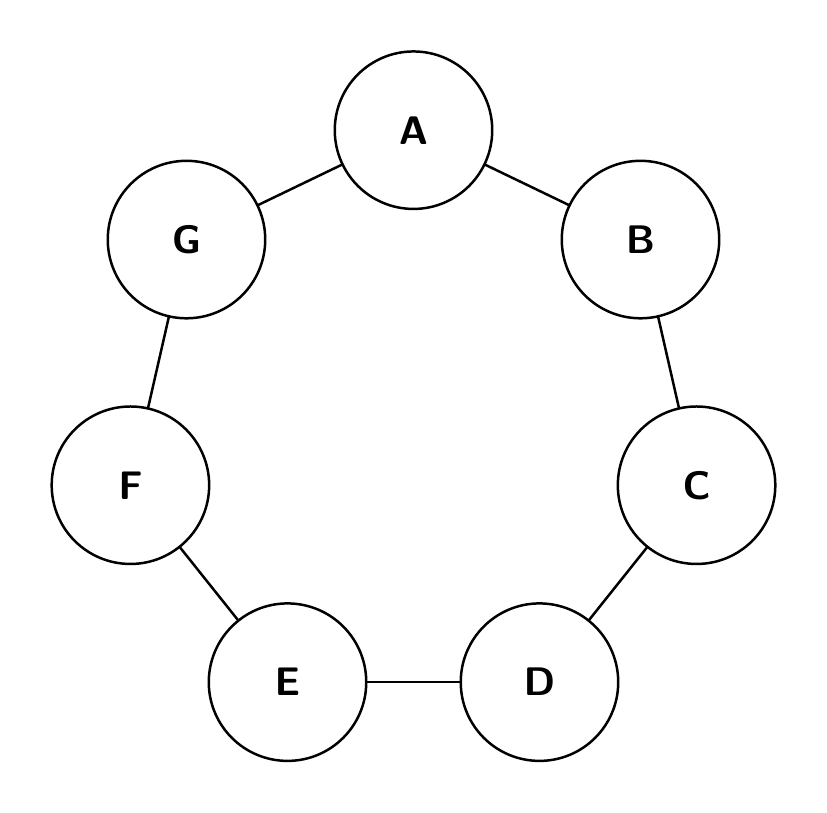
\begin{tikzpicture}[x=1mm, y=1mm]
\useasboundingbox (-49.0,-46.2) rectangle (49.0,49.9);
\draw[line width=0.9pt] (0.00,36.88) -- (28.83,22.99);
\draw[line width=0.9pt] (28.83,22.99) -- (35.95,-8.21);
\draw[line width=0.9pt] (35.95,-8.21) -- (16.00,-33.22);
\draw[line width=0.9pt] (16.00,-33.22) -- (-16.00,-33.22);
\draw[line width=0.9pt] (-16.00,-33.22) -- (-35.95,-8.21);
\draw[line width=0.9pt] (-35.95,-8.21) -- (-28.83,22.99);
\draw[line width=0.9pt] (-28.83,22.99) -- (0.00,36.88);
\draw[line width=0.9pt, fill=white] (0.00,36.88) circle (10.0mm);
\node[font=\Large\bfseries] at (0.00,36.88) {A};
\draw[line width=0.9pt, fill=white] (28.83,22.99) circle (10.0mm);
\node[font=\Large\bfseries] at (28.83,22.99) {B};
\draw[line width=0.9pt, fill=white] (35.95,-8.21) circle (10.0mm);
\node[font=\Large\bfseries] at (35.95,-8.21) {C};
\draw[line width=0.9pt, fill=white] (16.00,-33.22) circle (10.0mm);
\node[font=\Large\bfseries] at (16.00,-33.22) {D};
\draw[line width=0.9pt, fill=white] (-16.00,-33.22) circle (10.0mm);
\node[font=\Large\bfseries] at (-16.00,-33.22) {E};
\draw[line width=0.9pt, fill=white] (-35.95,-8.21) circle (10.0mm);
\node[font=\Large\bfseries] at (-35.95,-8.21) {F};
\draw[line width=0.9pt, fill=white] (-28.83,22.99) circle (10.0mm);
\node[font=\Large\bfseries] at (-28.83,22.99) {G};
\end{tikzpicture} \hfill}\par
\newpage
\textbf{Problem 7:} Use counters 1, 2 and 3, and begin at Start each time. Which goals can you reach? Write your moves. For a goal you can't reach, explain why.\par
\vspace{8mm}
\noindent\makebox[\linewidth][c]{\begin{tikzpicture}[x=1mm, y=1mm]
\useasboundingbox (-40.1,-83.4) rectangle (131.9,60.3);
\draw[line width=0.9pt] (0.00,30.62) -- (29.12,9.46);
\draw[line width=0.9pt] (29.12,9.46) -- (18.00,-24.77);
\draw[line width=0.9pt] (18.00,-24.77) -- (-18.00,-24.77);
\draw[line width=0.9pt] (-18.00,-24.77) -- (-29.12,9.46);
\draw[line width=0.9pt] (-29.12,9.46) -- (0.00,30.62);
\draw[line width=0.9pt, fill=white] (0.00,30.62) circle (10.0mm);
\node[font=\Large\bfseries] at (0.00,30.62) {A};
\draw[line width=0.9pt, fill=white] (29.12,9.46) circle (10.0mm);
\node[font=\Large\bfseries] at (29.12,9.46) {B};
\draw[line width=0.9pt, fill=white] (18.00,-24.77) circle (10.0mm);
\node[font=\Large\bfseries] at (18.00,-24.77) {C};
\draw[line width=0.9pt, fill=white] (-18.00,-24.77) circle (10.0mm);
\node[font=\Large\bfseries] at (-18.00,-24.77) {D};
\draw[line width=0.9pt, fill=white] (-29.12,9.46) circle (10.0mm);
\node[font=\Large\bfseries] at (-29.12,9.46) {E};
\node[anchor=north west, font=\small\bfseries, inner sep=0] at (51.1,59.3) {Start};
\draw[line width=0.7pt] (66.16,47.95) -- (74.90,41.61);
\draw[line width=0.7pt] (74.90,41.61) -- (71.56,31.33);
\draw[line width=0.7pt] (71.56,31.33) -- (60.76,31.33);
\draw[line width=0.7pt] (60.76,31.33) -- (57.42,41.61);
\draw[line width=0.7pt] (57.42,41.61) -- (66.16,47.95);
\draw[line width=0.7pt, fill=white] (66.16,47.95) circle (3.8mm);
\node[font=\small\bfseries] at (66.16,47.95) {1};
\node[font=\scriptsize, inner sep=0.4mm, anchor=270] at (66.16,52.25) {A};
\draw[line width=0.7pt, fill=white] (74.90,41.61) circle (3.8mm);
\node[font=\small\bfseries] at (74.90,41.61) {2};
\node[font=\scriptsize, inner sep=0.4mm, anchor=225] at (77.94,44.65) {B};
\draw[line width=0.7pt, fill=white] (71.56,31.33) circle (3.8mm);
\node[font=\small\bfseries] at (71.56,31.33) {3};
\node[font=\scriptsize, inner sep=0.4mm, anchor=90] at (71.56,27.03) {C};
\draw[line width=0.7pt, fill=white] (60.76,31.33) circle (3.8mm);
\node[font=\small\bfseries] at (60.76,31.33) {1};
\node[font=\scriptsize, inner sep=0.4mm, anchor=30] at (57.04,29.18) {D};
\draw[line width=0.7pt, fill=white] (57.42,41.61) circle (3.8mm);
\node[font=\small\bfseries] at (57.42,41.61) {2};
\node[font=\scriptsize, inner sep=0.4mm, anchor=315] at (54.38,44.65) {E};
\node[anchor=north west, font=\small\bfseries, inner sep=0] at (51.1,20.0) {Goal 1};
\draw[line width=0.7pt] (66.16,8.73) -- (74.90,2.39);
\draw[line width=0.7pt] (74.90,2.39) -- (71.56,-7.89);
\draw[line width=0.7pt] (71.56,-7.89) -- (60.76,-7.89);
\draw[line width=0.7pt] (60.76,-7.89) -- (57.42,2.39);
\draw[line width=0.7pt] (57.42,2.39) -- (66.16,8.73);
\draw[line width=0.7pt, fill=white] (66.16,8.73) circle (3.8mm);
\node[font=\small\bfseries] at (66.16,8.73) {2};
\node[font=\scriptsize, inner sep=0.4mm, anchor=270] at (66.16,13.03) {A};
\draw[line width=0.7pt, fill=white] (74.90,2.39) circle (3.8mm);
\node[font=\small\bfseries] at (74.90,2.39) {3};
\node[font=\scriptsize, inner sep=0.4mm, anchor=225] at (77.94,5.43) {B};
\draw[line width=0.7pt, fill=white] (71.56,-7.89) circle (3.8mm);
\node[font=\small\bfseries] at (71.56,-7.89) {1};
\node[font=\scriptsize, inner sep=0.4mm, anchor=90] at (71.56,-12.19) {C};
\draw[line width=0.7pt, fill=white] (60.76,-7.89) circle (3.8mm);
\node[font=\small\bfseries] at (60.76,-7.89) {2};
\node[font=\scriptsize, inner sep=0.4mm, anchor=30] at (57.04,-10.04) {D};
\draw[line width=0.7pt, fill=white] (57.42,2.39) circle (3.8mm);
\node[font=\small\bfseries] at (57.42,2.39) {3};
\node[font=\scriptsize, inner sep=0.4mm, anchor=315] at (54.38,5.43) {E};
\node[anchor=north west, font=\small\bfseries, inner sep=0] at (51.1,-19.2) {Goal 2};
\draw[line width=0.7pt] (66.16,-30.49) -- (74.90,-36.83);
\draw[line width=0.7pt] (74.90,-36.83) -- (71.56,-47.10);
\draw[line width=0.7pt] (71.56,-47.10) -- (60.76,-47.10);
\draw[line width=0.7pt] (60.76,-47.10) -- (57.42,-36.83);
\draw[line width=0.7pt] (57.42,-36.83) -- (66.16,-30.49);
\draw[line width=0.7pt, fill=white] (66.16,-30.49) circle (3.8mm);
\node[font=\small\bfseries] at (66.16,-30.49) {1};
\node[font=\scriptsize, inner sep=0.4mm, anchor=270] at (66.16,-26.19) {A};
\draw[line width=0.7pt, fill=white] (74.90,-36.83) circle (3.8mm);
\node[font=\small\bfseries] at (74.90,-36.83) {3};
\node[font=\scriptsize, inner sep=0.4mm, anchor=225] at (77.94,-33.79) {B};
\draw[line width=0.7pt, fill=white] (71.56,-47.10) circle (3.8mm);
\node[font=\small\bfseries] at (71.56,-47.10) {2};
\node[font=\scriptsize, inner sep=0.4mm, anchor=90] at (71.56,-51.40) {C};
\draw[line width=0.7pt, fill=white] (60.76,-47.10) circle (3.8mm);
\node[font=\small\bfseries] at (60.76,-47.10) {1};
\node[font=\scriptsize, inner sep=0.4mm, anchor=30] at (57.04,-49.25) {D};
\draw[line width=0.7pt, fill=white] (57.42,-36.83) circle (3.8mm);
\node[font=\small\bfseries] at (57.42,-36.83) {3};
\node[font=\scriptsize, inner sep=0.4mm, anchor=315] at (54.38,-33.79) {E};
\node[anchor=west, font=\small] at (-39.1,-67.4) {Goal 1:};
\draw[line width=0.5pt] (-22.1,-69.4) -- (130.9,-69.4);
\node[anchor=west, font=\small] at (-39.1,-79.4) {Goal 2:};
\draw[line width=0.5pt] (-22.1,-81.4) -- (130.9,-81.4);
\end{tikzpicture}}\par
\newpage
\textbf{Problem 8:} Now counter 4 may be used too. Change Start into Goal in as few moves as you can. On a ring of any size, with counters 1, 2, 3, 4, can every placement with different numbers at the two ends of every line be changed into every other one? Explain.\par
\vspace{10mm}
\noindent\makebox[\linewidth][c]{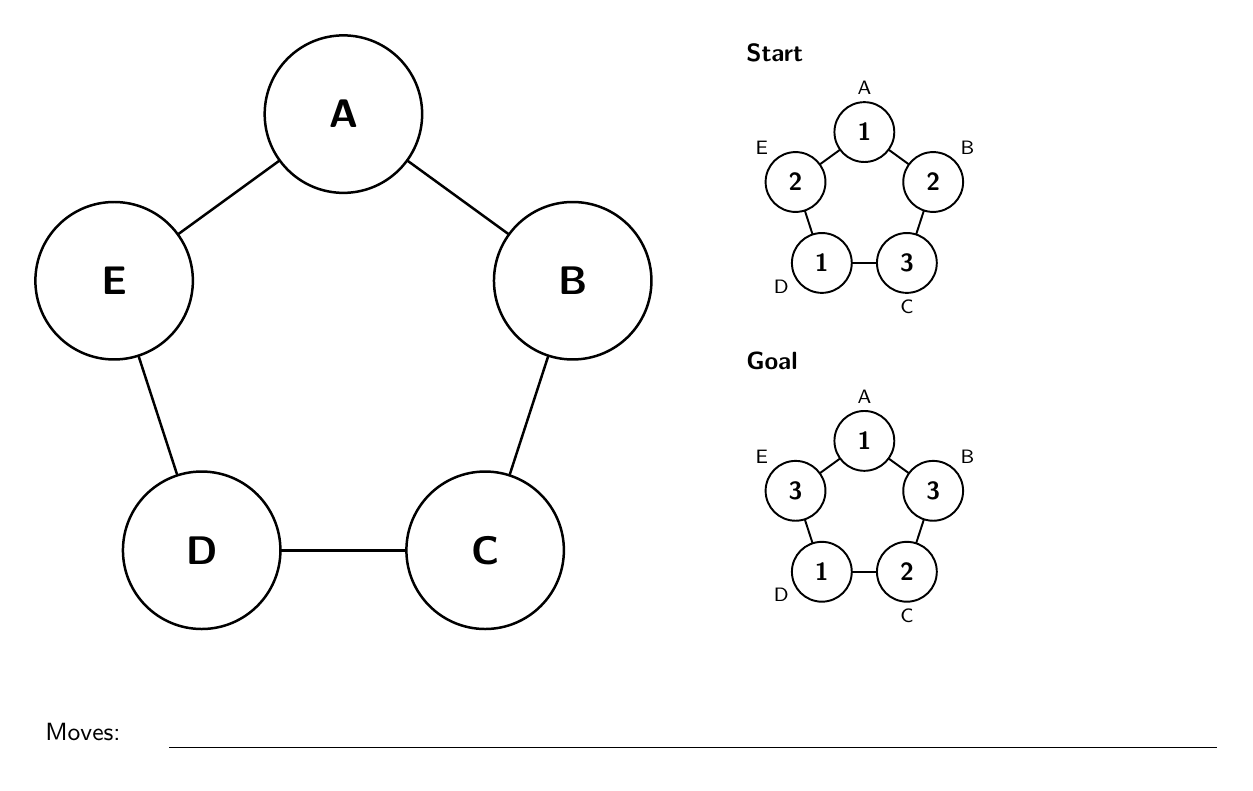
\begin{tikzpicture}[x=1mm, y=1mm]
\useasboundingbox (-40.1,-51.8) rectangle (111.9,41.6);
\draw[line width=0.9pt] (0.00,30.62) -- (29.12,9.46);
\draw[line width=0.9pt] (29.12,9.46) -- (18.00,-24.77);
\draw[line width=0.9pt] (18.00,-24.77) -- (-18.00,-24.77);
\draw[line width=0.9pt] (-18.00,-24.77) -- (-29.12,9.46);
\draw[line width=0.9pt] (-29.12,9.46) -- (0.00,30.62);
\draw[line width=0.9pt, fill=white] (0.00,30.62) circle (10.0mm);
\node[font=\Large\bfseries] at (0.00,30.62) {A};
\draw[line width=0.9pt, fill=white] (29.12,9.46) circle (10.0mm);
\node[font=\Large\bfseries] at (29.12,9.46) {B};
\draw[line width=0.9pt, fill=white] (18.00,-24.77) circle (10.0mm);
\node[font=\Large\bfseries] at (18.00,-24.77) {C};
\draw[line width=0.9pt, fill=white] (-18.00,-24.77) circle (10.0mm);
\node[font=\Large\bfseries] at (-18.00,-24.77) {D};
\draw[line width=0.9pt, fill=white] (-29.12,9.46) circle (10.0mm);
\node[font=\Large\bfseries] at (-29.12,9.46) {E};
\node[anchor=north west, font=\small\bfseries, inner sep=0] at (51.1,39.6) {Start};
\draw[line width=0.7pt] (66.16,28.34) -- (74.90,22.00);
\draw[line width=0.7pt] (74.90,22.00) -- (71.56,11.72);
\draw[line width=0.7pt] (71.56,11.72) -- (60.76,11.72);
\draw[line width=0.7pt] (60.76,11.72) -- (57.42,22.00);
\draw[line width=0.7pt] (57.42,22.00) -- (66.16,28.34);
\draw[line width=0.7pt, fill=white] (66.16,28.34) circle (3.8mm);
\node[font=\small\bfseries] at (66.16,28.34) {1};
\node[font=\scriptsize, inner sep=0.4mm, anchor=270] at (66.16,32.64) {A};
\draw[line width=0.7pt, fill=white] (74.90,22.00) circle (3.8mm);
\node[font=\small\bfseries] at (74.90,22.00) {2};
\node[font=\scriptsize, inner sep=0.4mm, anchor=225] at (77.94,25.04) {B};
\draw[line width=0.7pt, fill=white] (71.56,11.72) circle (3.8mm);
\node[font=\small\bfseries] at (71.56,11.72) {3};
\node[font=\scriptsize, inner sep=0.4mm, anchor=90] at (71.56,7.42) {C};
\draw[line width=0.7pt, fill=white] (60.76,11.72) circle (3.8mm);
\node[font=\small\bfseries] at (60.76,11.72) {1};
\node[font=\scriptsize, inner sep=0.4mm, anchor=30] at (57.04,9.57) {D};
\draw[line width=0.7pt, fill=white] (57.42,22.00) circle (3.8mm);
\node[font=\small\bfseries] at (57.42,22.00) {2};
\node[font=\scriptsize, inner sep=0.4mm, anchor=315] at (54.38,25.04) {E};
\node[anchor=north west, font=\small\bfseries, inner sep=0] at (51.1,0.4) {Goal};
\draw[line width=0.7pt] (66.16,-10.88) -- (74.90,-17.22);
\draw[line width=0.7pt] (74.90,-17.22) -- (71.56,-27.50);
\draw[line width=0.7pt] (71.56,-27.50) -- (60.76,-27.50);
\draw[line width=0.7pt] (60.76,-27.50) -- (57.42,-17.22);
\draw[line width=0.7pt] (57.42,-17.22) -- (66.16,-10.88);
\draw[line width=0.7pt, fill=white] (66.16,-10.88) circle (3.8mm);
\node[font=\small\bfseries] at (66.16,-10.88) {1};
\node[font=\scriptsize, inner sep=0.4mm, anchor=270] at (66.16,-6.58) {A};
\draw[line width=0.7pt, fill=white] (74.90,-17.22) circle (3.8mm);
\node[font=\small\bfseries] at (74.90,-17.22) {3};
\node[font=\scriptsize, inner sep=0.4mm, anchor=225] at (77.94,-14.18) {B};
\draw[line width=0.7pt, fill=white] (71.56,-27.50) circle (3.8mm);
\node[font=\small\bfseries] at (71.56,-27.50) {2};
\node[font=\scriptsize, inner sep=0.4mm, anchor=90] at (71.56,-31.80) {C};
\draw[line width=0.7pt, fill=white] (60.76,-27.50) circle (3.8mm);
\node[font=\small\bfseries] at (60.76,-27.50) {1};
\node[font=\scriptsize, inner sep=0.4mm, anchor=30] at (57.04,-29.65) {D};
\draw[line width=0.7pt, fill=white] (57.42,-17.22) circle (3.8mm);
\node[font=\small\bfseries] at (57.42,-17.22) {3};
\node[font=\scriptsize, inner sep=0.4mm, anchor=315] at (54.38,-14.18) {E};
\node[anchor=west, font=\small] at (-39.1,-47.8) {Moves:};
\draw[line width=0.5pt] (-22.1,-49.8) -- (110.9,-49.8);
\end{tikzpicture}}\par
\newpage
Lay the headers in a row, 1, 2, 3, 4, where 1 comes first. Put each card under a header, and a counter with that header's number on the card's circle. An arrow from one card to another means the first card must come earlier, under a smaller number. Cards with no arrow between them may share a header.\par
\vspace{3mm}
\noindent\makebox[\linewidth][c]{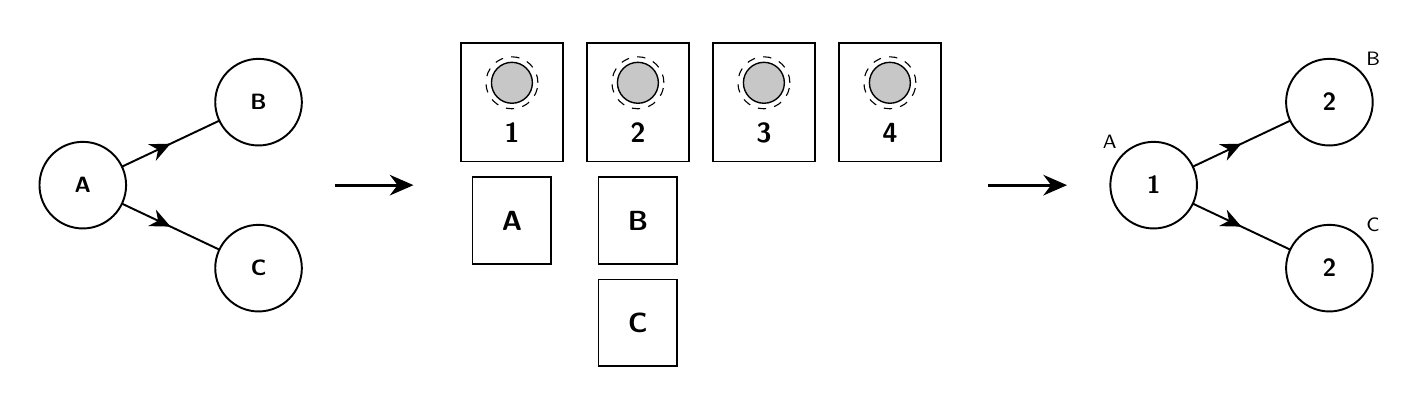
\begin{tikzpicture}[x=1mm, y=1mm]
\useasboundingbox (-7.0,-24.0) rectangle (167.0,20.0);
\draw[line width=0.7pt,smallarrow] (0.00,0.00) -- (22.32,10.54);
\draw[line width=0.7pt,smallarrow] (0.00,0.00) -- (22.32,-10.54);
\draw[line width=0.7pt, fill=white] (0.00,0.00) circle (5.5mm);
\node[font=\footnotesize\bfseries] at (0.00,0.00) {A};
\draw[line width=0.7pt, fill=white] (22.32,10.54) circle (5.5mm);
\node[font=\footnotesize\bfseries] at (22.32,10.54) {B};
\draw[line width=0.7pt, fill=white] (22.32,-10.54) circle (5.5mm);
\node[font=\footnotesize\bfseries] at (22.32,-10.54) {C};
\draw[bigarrow] (32,0) -- (42,0);
\draw[line width=0.7pt, fill=white] (48.0,3.0) rectangle (61.0,18.0);
\draw[dashed, line width=0.4pt] (54.5,13.0) circle (3.3mm);
\draw[line width=0.5pt, fill=black!22] (54.5,13.0) circle (2.6mm);
\node[font=\bfseries] at (54.5,6.6) {1};
\draw[line width=0.7pt, fill=white] (64.0,3.0) rectangle (77.0,18.0);
\draw[dashed, line width=0.4pt] (70.5,13.0) circle (3.3mm);
\draw[line width=0.5pt, fill=black!22] (70.5,13.0) circle (2.6mm);
\node[font=\bfseries] at (70.5,6.6) {2};
\draw[line width=0.7pt, fill=white] (80.0,3.0) rectangle (93.0,18.0);
\draw[dashed, line width=0.4pt] (86.5,13.0) circle (3.3mm);
\draw[line width=0.5pt, fill=black!22] (86.5,13.0) circle (2.6mm);
\node[font=\bfseries] at (86.5,6.6) {3};
\draw[line width=0.7pt, fill=white] (96.0,3.0) rectangle (109.0,18.0);
\draw[dashed, line width=0.4pt] (102.5,13.0) circle (3.3mm);
\draw[line width=0.5pt, fill=black!22] (102.5,13.0) circle (2.6mm);
\node[font=\bfseries] at (102.5,6.6) {4};
\draw[line width=0.6pt, fill=white] (49.5,-10.0) rectangle (59.5,1.0);
\node[font=\bfseries] at (54.5,-4.5) {A};
\draw[line width=0.6pt, fill=white] (65.5,-10.0) rectangle (75.5,1.0);
\node[font=\bfseries] at (70.5,-4.5) {B};
\draw[line width=0.6pt, fill=white] (65.5,-23.0) rectangle (75.5,-12.0);
\node[font=\bfseries] at (70.5,-17.5) {C};
\draw[bigarrow] (115.0,0) -- (125.0,0);
\draw[line width=0.7pt,smallarrow] (136.00,0.00) -- (158.32,10.54);
\draw[line width=0.7pt,smallarrow] (136.00,0.00) -- (158.32,-10.54);
\draw[line width=0.7pt, fill=white] (136.00,0.00) circle (5.5mm);
\node[font=\small\bfseries] at (136.00,0.00) {1};
\node[font=\scriptsize, inner sep=0.4mm, anchor=315] at (131.76,4.24) {A};
\draw[line width=0.7pt, fill=white] (158.32,10.54) circle (5.5mm);
\node[font=\small\bfseries] at (158.32,10.54) {2};
\node[font=\scriptsize, inner sep=0.4mm, anchor=225] at (162.56,14.78) {B};
\draw[line width=0.7pt, fill=white] (158.32,-10.54) circle (5.5mm);
\node[font=\small\bfseries] at (158.32,-10.54) {2};
\node[font=\scriptsize, inner sep=0.4mm, anchor=225] at (162.56,-6.30) {C};
\end{tikzpicture}}\par
\vspace{4mm}
\textbf{Problem 9:} Put every card under a header, using as few headers as you can. Explain why fewer headers can't work.\par
\vspace{10mm}
\noindent\makebox[\linewidth][c]{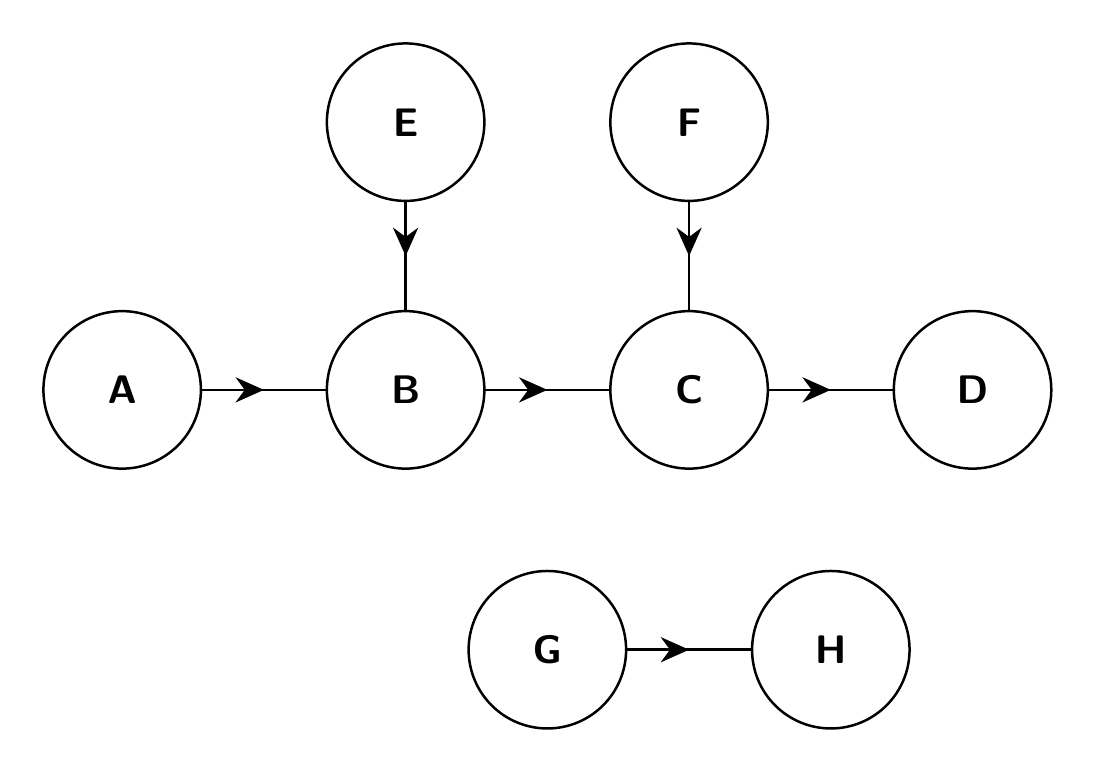
\begin{tikzpicture}[x=1mm, y=1mm]
\useasboundingbox (-12.0,-45.0) rectangle (120.0,46.0);
\draw[line width=0.9pt,midarrow] (0.00,0.00) -- (36.00,0.00);
\draw[line width=0.9pt,midarrow] (36.00,0.00) -- (72.00,0.00);
\draw[line width=0.9pt,midarrow] (72.00,0.00) -- (108.00,0.00);
\draw[line width=0.9pt,midarrow] (36.00,34.00) -- (36.00,0.00);
\draw[line width=0.9pt,midarrow] (72.00,34.00) -- (72.00,0.00);
\draw[line width=0.9pt,midarrow] (54.00,-33.00) -- (90.00,-33.00);
\draw[line width=0.9pt, fill=white] (0.00,0.00) circle (10.0mm);
\node[font=\Large\bfseries] at (0.00,0.00) {A};
\draw[line width=0.9pt, fill=white] (36.00,0.00) circle (10.0mm);
\node[font=\Large\bfseries] at (36.00,0.00) {B};
\draw[line width=0.9pt, fill=white] (72.00,0.00) circle (10.0mm);
\node[font=\Large\bfseries] at (72.00,0.00) {C};
\draw[line width=0.9pt, fill=white] (108.00,0.00) circle (10.0mm);
\node[font=\Large\bfseries] at (108.00,0.00) {D};
\draw[line width=0.9pt, fill=white] (36.00,34.00) circle (10.0mm);
\node[font=\Large\bfseries] at (36.00,34.00) {E};
\draw[line width=0.9pt, fill=white] (72.00,34.00) circle (10.0mm);
\node[font=\Large\bfseries] at (72.00,34.00) {F};
\draw[line width=0.9pt, fill=white] (54.00,-33.00) circle (10.0mm);
\node[font=\Large\bfseries] at (54.00,-33.00) {G};
\draw[line width=0.9pt, fill=white] (90.00,-33.00) circle (10.0mm);
\node[font=\Large\bfseries] at (90.00,-33.00) {H};
\end{tikzpicture}}\par
\newpage
\textbf{Problem 10:} Can the cards of each network be put under the four headers?\par
\vspace{10mm}
\noindent\makebox[\linewidth][c]{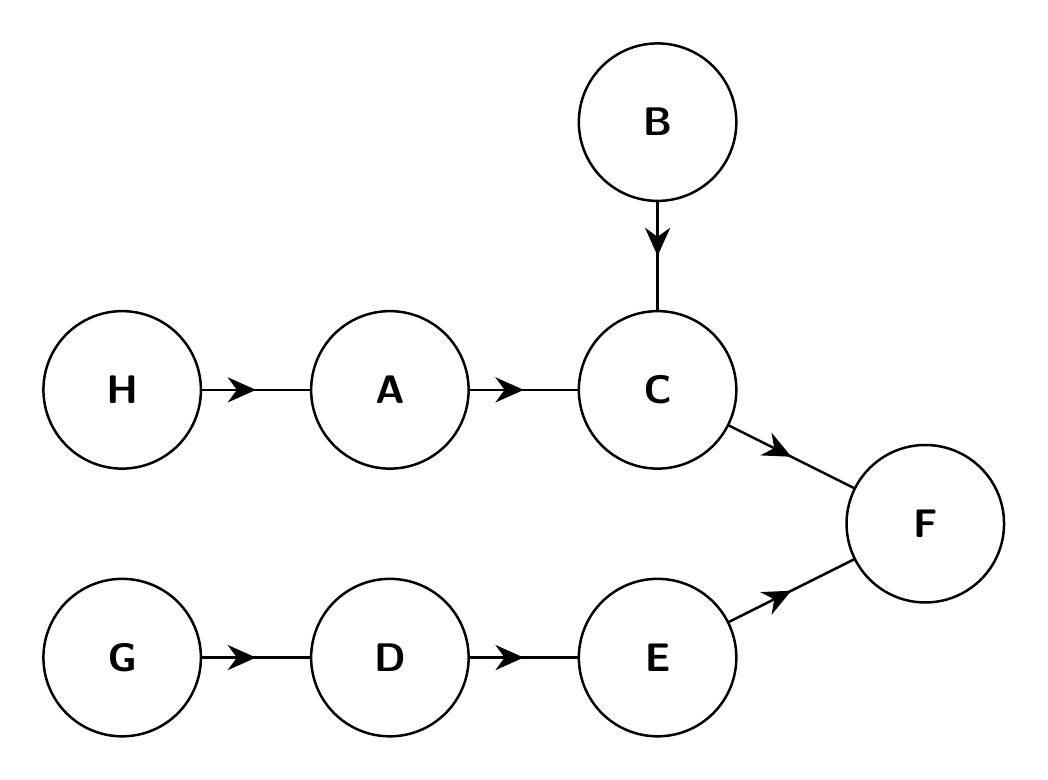
\begin{tikzpicture}[x=1mm, y=1mm]
\useasboundingbox (-12.0,-12.0) rectangle (114.0,80.0);
\draw[line width=0.9pt,midarrow] (0.00,34.00) -- (34.00,34.00);
\draw[line width=0.9pt,midarrow] (34.00,34.00) -- (68.00,34.00);
\draw[line width=0.9pt,midarrow] (68.00,68.00) -- (68.00,34.00);
\draw[line width=0.9pt,midarrow] (68.00,34.00) -- (102.00,17.00);
\draw[line width=0.9pt,midarrow] (0.00,0.00) -- (34.00,0.00);
\draw[line width=0.9pt,midarrow] (34.00,0.00) -- (68.00,0.00);
\draw[line width=0.9pt,midarrow] (68.00,0.00) -- (102.00,17.00);
\draw[line width=0.9pt, fill=white] (0.00,34.00) circle (10.0mm);
\node[font=\Large\bfseries] at (0.00,34.00) {H};
\draw[line width=0.9pt, fill=white] (34.00,34.00) circle (10.0mm);
\node[font=\Large\bfseries] at (34.00,34.00) {A};
\draw[line width=0.9pt, fill=white] (68.00,34.00) circle (10.0mm);
\node[font=\Large\bfseries] at (68.00,34.00) {C};
\draw[line width=0.9pt, fill=white] (102.00,17.00) circle (10.0mm);
\node[font=\Large\bfseries] at (102.00,17.00) {F};
\draw[line width=0.9pt, fill=white] (0.00,0.00) circle (10.0mm);
\node[font=\Large\bfseries] at (0.00,0.00) {G};
\draw[line width=0.9pt, fill=white] (34.00,0.00) circle (10.0mm);
\node[font=\Large\bfseries] at (34.00,0.00) {D};
\draw[line width=0.9pt, fill=white] (68.00,0.00) circle (10.0mm);
\node[font=\Large\bfseries] at (68.00,0.00) {E};
\draw[line width=0.9pt, fill=white] (68.00,68.00) circle (10.0mm);
\node[font=\Large\bfseries] at (68.00,68.00) {B};
\end{tikzpicture}}\par
\vspace{16mm}
\noindent\makebox[\linewidth][c]{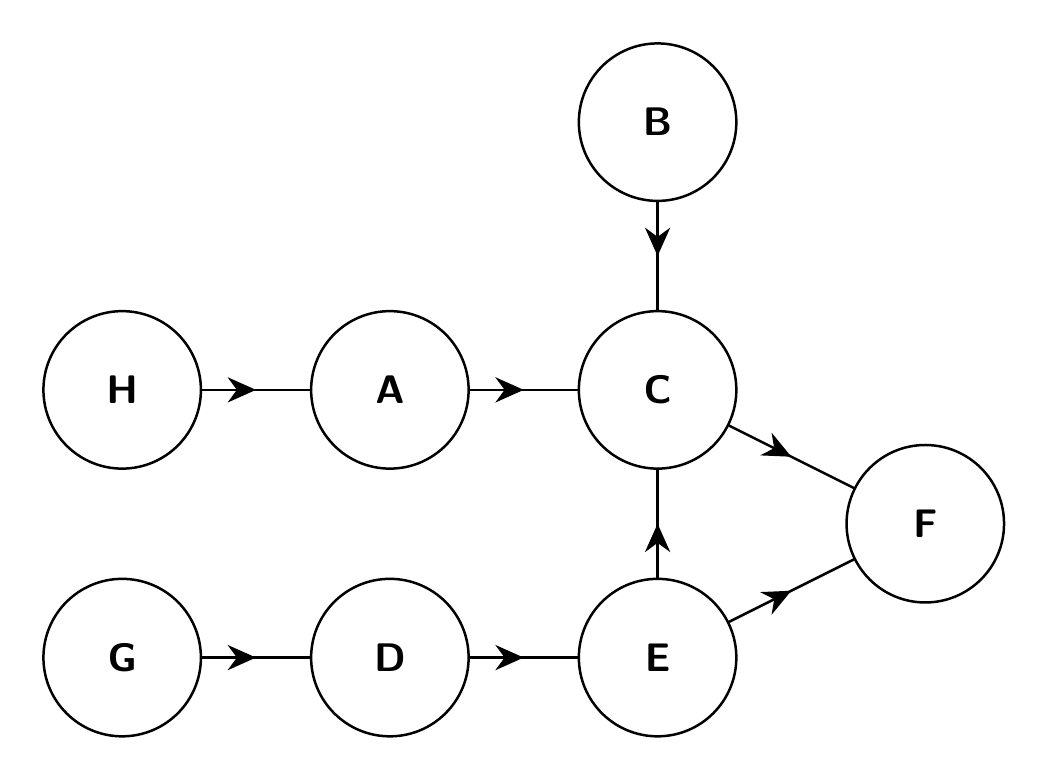
\begin{tikzpicture}[x=1mm, y=1mm]
\useasboundingbox (-12.0,-12.0) rectangle (114.0,80.0);
\draw[line width=0.9pt,midarrow] (0.00,34.00) -- (34.00,34.00);
\draw[line width=0.9pt,midarrow] (34.00,34.00) -- (68.00,34.00);
\draw[line width=0.9pt,midarrow] (68.00,68.00) -- (68.00,34.00);
\draw[line width=0.9pt,midarrow] (68.00,34.00) -- (102.00,17.00);
\draw[line width=0.9pt,midarrow] (0.00,0.00) -- (34.00,0.00);
\draw[line width=0.9pt,midarrow] (34.00,0.00) -- (68.00,0.00);
\draw[line width=0.9pt,midarrow] (68.00,0.00) -- (102.00,17.00);
\draw[line width=0.9pt,midarrow] (68.00,0.00) -- (68.00,34.00);
\draw[line width=0.9pt, fill=white] (0.00,34.00) circle (10.0mm);
\node[font=\Large\bfseries] at (0.00,34.00) {H};
\draw[line width=0.9pt, fill=white] (34.00,34.00) circle (10.0mm);
\node[font=\Large\bfseries] at (34.00,34.00) {A};
\draw[line width=0.9pt, fill=white] (68.00,34.00) circle (10.0mm);
\node[font=\Large\bfseries] at (68.00,34.00) {C};
\draw[line width=0.9pt, fill=white] (102.00,17.00) circle (10.0mm);
\node[font=\Large\bfseries] at (102.00,17.00) {F};
\draw[line width=0.9pt, fill=white] (0.00,0.00) circle (10.0mm);
\node[font=\Large\bfseries] at (0.00,0.00) {G};
\draw[line width=0.9pt, fill=white] (34.00,0.00) circle (10.0mm);
\node[font=\Large\bfseries] at (34.00,0.00) {D};
\draw[line width=0.9pt, fill=white] (68.00,0.00) circle (10.0mm);
\node[font=\Large\bfseries] at (68.00,0.00) {E};
\draw[line width=0.9pt, fill=white] (68.00,68.00) circle (10.0mm);
\node[font=\Large\bfseries] at (68.00,68.00) {B};
\end{tikzpicture}}\par
\newpage
\textbf{Problem 11:} Draw an arrowhead on every line so that the longest path along the arrows passes through as few cards as you can. Then put the cards under headers to follow your arrows. On the first network, can you draw the arrows so that no path along the arrows passes through three cards? Explain.\par
\vspace{6mm}
\noindent\makebox[\linewidth][c]{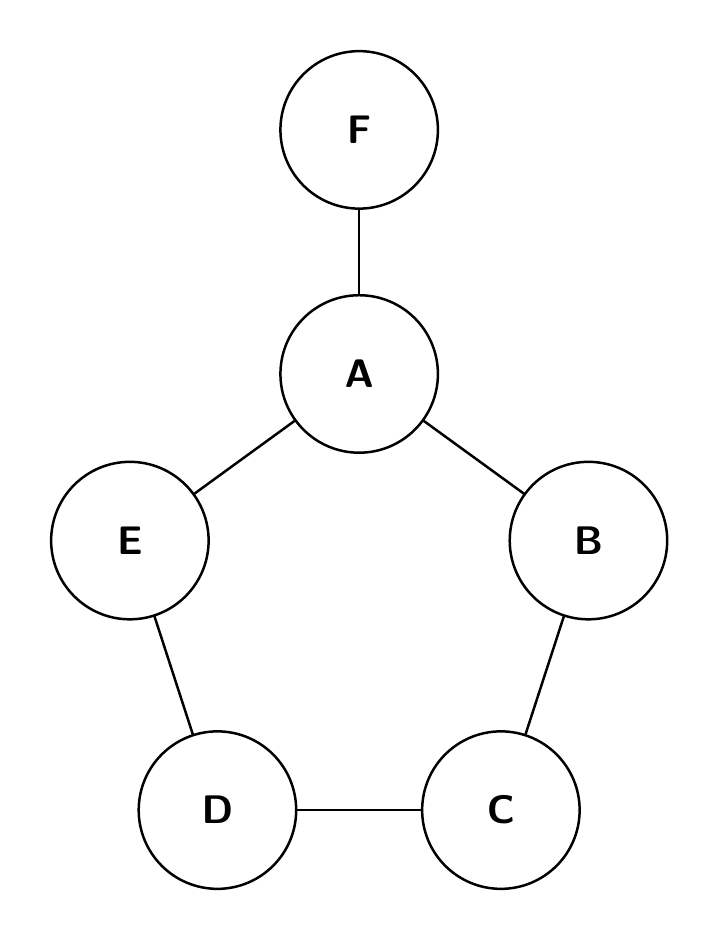
\begin{tikzpicture}[x=1mm, y=1mm]
\useasboundingbox (-42.1,-37.8) rectangle (42.1,74.6);
\draw[line width=0.9pt] (0.00,30.62) -- (29.12,9.46);
\draw[line width=0.9pt] (29.12,9.46) -- (18.00,-24.77);
\draw[line width=0.9pt] (18.00,-24.77) -- (-18.00,-24.77);
\draw[line width=0.9pt] (-18.00,-24.77) -- (-29.12,9.46);
\draw[line width=0.9pt] (-29.12,9.46) -- (0.00,30.62);
\draw[line width=0.9pt] (0.00,30.62) -- (0.00,61.62);
\draw[line width=0.9pt, fill=white] (0.00,30.62) circle (10.0mm);
\node[font=\Large\bfseries] at (0.00,30.62) {A};
\draw[line width=0.9pt, fill=white] (29.12,9.46) circle (10.0mm);
\node[font=\Large\bfseries] at (29.12,9.46) {B};
\draw[line width=0.9pt, fill=white] (18.00,-24.77) circle (10.0mm);
\node[font=\Large\bfseries] at (18.00,-24.77) {C};
\draw[line width=0.9pt, fill=white] (-18.00,-24.77) circle (10.0mm);
\node[font=\Large\bfseries] at (-18.00,-24.77) {D};
\draw[line width=0.9pt, fill=white] (-29.12,9.46) circle (10.0mm);
\node[font=\Large\bfseries] at (-29.12,9.46) {E};
\draw[line width=0.9pt, fill=white] (0.00,61.62) circle (10.0mm);
\node[font=\Large\bfseries] at (0.00,61.62) {F};
\end{tikzpicture}}\par
\vspace{8mm}
\noindent\makebox[\linewidth][c]{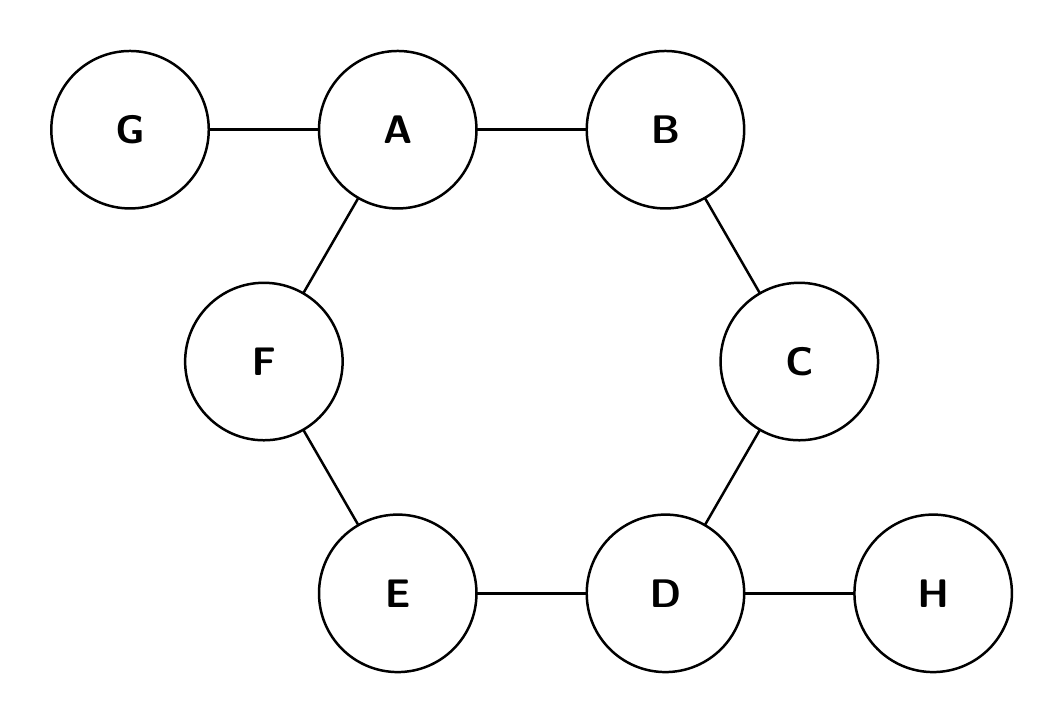
\begin{tikzpicture}[x=1mm, y=1mm]
\useasboundingbox (-64.0,-42.4) rectangle (64.0,42.4);
\draw[line width=0.9pt] (-17.00,29.44) -- (17.00,29.44);
\draw[line width=0.9pt] (17.00,29.44) -- (34.00,0.00);
\draw[line width=0.9pt] (34.00,0.00) -- (17.00,-29.44);
\draw[line width=0.9pt] (17.00,-29.44) -- (-17.00,-29.44);
\draw[line width=0.9pt] (-17.00,-29.44) -- (-34.00,-0.00);
\draw[line width=0.9pt] (-34.00,-0.00) -- (-17.00,29.44);
\draw[line width=0.9pt] (-17.00,29.44) -- (-51.00,29.44);
\draw[line width=0.9pt] (17.00,-29.44) -- (51.00,-29.44);
\draw[line width=0.9pt, fill=white] (-17.00,29.44) circle (10.0mm);
\node[font=\Large\bfseries] at (-17.00,29.44) {A};
\draw[line width=0.9pt, fill=white] (17.00,29.44) circle (10.0mm);
\node[font=\Large\bfseries] at (17.00,29.44) {B};
\draw[line width=0.9pt, fill=white] (34.00,0.00) circle (10.0mm);
\node[font=\Large\bfseries] at (34.00,0.00) {C};
\draw[line width=0.9pt, fill=white] (17.00,-29.44) circle (10.0mm);
\node[font=\Large\bfseries] at (17.00,-29.44) {D};
\draw[line width=0.9pt, fill=white] (-17.00,-29.44) circle (10.0mm);
\node[font=\Large\bfseries] at (-17.00,-29.44) {E};
\draw[line width=0.9pt, fill=white] (-34.00,-0.00) circle (10.0mm);
\node[font=\Large\bfseries] at (-34.00,-0.00) {F};
\draw[line width=0.9pt, fill=white] (-51.00,29.44) circle (10.0mm);
\node[font=\Large\bfseries] at (-51.00,29.44) {G};
\draw[line width=0.9pt, fill=white] (51.00,-29.44) circle (10.0mm);
\node[font=\Large\bfseries] at (51.00,-29.44) {H};
\end{tikzpicture}}\par
\end{document}
